
\documentclass[conference,onecolumn]{IEEEtran}
%\documentclass[article,onecolumn]{IEEEtran}
\usepackage{cite}
\usepackage{amsmath,amssymb,amsfonts}
\usepackage{algorithmic}
\usepackage{graphicx}
\usepackage{textcomp}
\usepackage{xcolor}
\usepackage{float}
\usepackage{subcaption}
\usepackage{multirow}
\usepackage{colortbl}
\usepackage{tabularx}
\usepackage{color}
\usepackage{array}
\newcolumntype{P}[1]{>{\centering\arraybackslash}p{#1}}
\definecolor{yellow}{rgb}{0.85, 1,1}
\definecolor{pastleyellow}{rgb}{1, 0.98,0.63}
\setlength{\arrayrulewidth}{0.1mm}
\setlength{\tabcolsep}{6pt}
\setlength\headheight{10pt}


\setlength\parskip{1em plus 0.1em minus 0.2em}
\setlength\parindent{0pt}
%\usepackage{parskip} 
\setlength{\parskip}{8pt}
\usepackage{subcaption}
%\setlength\extrarowheight{5pt}
\renewcommand{\arraystretch}{1.5}

\begin{document}

\title{Assessing the User Experience: A Usability Report on Delta3 Gmbh Software\\}

\author{\IEEEauthorblockN{Akshay Chikhalkar}\\
\IEEEauthorblockA{\textit{Department of Electrical Engineering and Computer Science} \\
\textit{Technische Hochschule Ostwestfalen-Lippe University of Applied Sciences and Arts}\\
Lemgo, Germany \\
akshay.chikhalkar@stud.th-owl.de}

}

\maketitle
		

\begin{abstract}
    This report explores software usability engineering, a critical aspect of software development that ensures the creation of easy-to-use, intuitive, and efficient software applications. It emphasizes the significance of software usability and identifies the factors that influence it. The report features a case study of Delta3 GmbH, a German software development company specializing in 3D scanning and modeling software. The study, conducted in both English and German, involved heuristic evaluation, usability testing, and a user experience questionnaire for three software products developed by Delta3 GmbH. Participants from different professions, age groups, and educational backgrounds who were unfamiliar with the software were recruited for the study. The report presents the study's findings, identifying the strengths and weaknesses of the products and analyzing the user experience questionnaire.
\end{abstract}

% Note that keywords are not normally used for peerreview papers.
\begin{IEEEkeywords}
	User experience questionnaire (UEQ), Usability Testing, Heuristic Evaluation, App / Player, Editor, Operations, User observations.
\end{IEEEkeywords}

\newpage
\tableofcontents

\newpage
\section{Introduction}

	The software usability engineering is a critical aspect of software development that focuses on designing and developing software applications that are easy to use, intuitive, and efficient \cite{dillon2001evaluation}. The success of a software product heavily depends on its usability and how well it meets the needs of its intended users \cite{berkman2016re}. Usability is determined by several factors, including interface design, instructions and documentation, performance, and reliability. Usability testing, heuristic evaluation, and user experience questionnaire are common method used to assess the usability of software products and make necessary improvements \cite{sagar2017systematic}.

	In this report, we will explore the importance of software usability engineering in more detail. We will discuss the various factors that influence software usability and the methods used to evaluate and improve it. Additionally, we will delve into the specific case of Delta3 GmbH, a software development company based in Germany that specializes in 3D scanning and modeling software solutions for various industries. We will examine their software products usability.

	Furthermore, we will discuss the study conducted on the three software products developed by Delta3 GmbH, which is divided into three parts: heuristic evaluation, usability testing,  and user experience questionnaire. The heuristic evaluation was based on 10 heuristic principles, while the user study involved five participants from different professions. We will discuss the results of the study, including the strengths and weaknesses of the software products and the improvements that can be made to enhance their usability.

\section{Evaluation methods}

    Software usability can be evaluated using various methods, such as usability testing, heuristic evaluation, cognitive walkthrough, expert review, survey/questionnaire, user interviews, and field studies \cite{sauro2012standardized}. Usability testing involves participants performing tasks while being observed by researchers to identify usability issues and gather feedback. Heuristic evaluation involves a group of experts evaluating the software based on established usability principles \cite{rubin2008handbook}. Cognitive walkthrough involves evaluators taking the perspective of users and walking through the steps required to complete a task to identify potential usability issues \cite{albert2013measuring}. Survey/questionnaire involves users providing feedback on their experience using the software through a series of prompts. User interviews involve asking users open-ended questions about their experience with the software to gather detailed feedback. Field studies involve observing users in their natural environment while using the software to identify usability issues \cite{sauro2016quantifying}.

    Each evaluation method has its own strengths and weaknesses, and the choice of method depends on factors such as the stage of development, evaluation goals, and available resources. Combining multiple methods can provide a more comprehensive understanding of software usability \cite{hartson2012ux}. For this particular study, heuristic evaluation, usability testing and user experience questionnaire are being used.

	\subsection{Heuristic Evaluation}
        Heuristic evaluation is a method used to systematically evaluate the usability of a user interface or product by a small group of evaluators \cite{nielsen1994heuristic}. These evaluators consist of individuals with relevant experience and expertise in usability, interaction design, and related fields. The evaluation process involves examining the interface against a set of predefined usability heuristics or guidelines that have been established through research and experience \cite{nielsen1994heuristic}.

        During the evaluation process, the evaluators identify any usability issues that violate the established heuristics and may provide recommendations to improve the interface's usability. This evaluation can be conducted at various stages of the design process, ranging from early wireframes to the final product.
        
        Heuristic evaluation offers a quick and cost-effective way to identify usability issues early on and provide feedback to improve the product's design \cite{molich1990improving}. This method can be useful in improving the usability of a product and ensuring a positive user experience.
        
        The evaluation of usability often involves the use of heuristic principles or guidelines that are established based on research and experience. Ten commonly used heuristic principles for evaluating usability are \cite{nielsen2005ten}:

        \begin{enumerate}
            \item Visibility of system status: The system should provide appropriate feedback within a reasonable amount of time to keep the user informed about what is happening.
            \item Match between system and the real world: The system should use words, phrases, and concepts that are familiar to the user, and follow real-world conventions.
            \item User control and freedom: Users should be provided with options to easily reverse actions and resume tasks.
            \item Consistency and standards: The system should follow platform conventions, and avoid confusing users with different words, situations, or actions.
            \item Error prevention: The system should be designed to prevent serious user mistakes by putting up constraints or barriers.
            \item Recognition rather than recall: The user should not have to remember information from one part of the interface to another, and objects, actions, and options should be visible.
            \item Flexibility and efficiency of use: The system should cater to both experienced and novice users, and allow the user to tailor frequent actions and automate repetitive tasks.
            \item Aesthetic and minimalist design: The interface should prioritize important information, and avoid containing irrelevant or rarely needed information.
            \item Help users recognize, diagnose, and recover from errors: Error messages should be expressed in plain language and clearly indicate the problem and steps to resolve it.    
            \item Help and documentation: The system should include documentation to help users understand features and capabilities, but the system should be designed in such a way that documentation is not needed to complete tasks.
        \end{enumerate}

        The use of these heuristic principles can help designers and evaluators identify usability issues and improve the overall user experience of a software application \cite{nielsen1994heuristic}.

    \subsection{Usability Testing}
        
        \subsubsection{User profiles}\hfill

            In the context of software usability, a user profile refers to a detailed depiction of the characteristics that define the typical or intended user for a specific software system \cite{molich1990improving}. This may include the user's demographic information, educational background, professional role, experience level, and any other pertinent factors that may influence their interaction with the software \cite{molich1990improving}.

            Creating a user profile is a crucial aspect of software usability design and evaluation, as it enables developers and designers to gain a better understanding of their target users' requirements and needs. By taking into account the user profile, designers can ensure that the software is customized to meet the specific needs and preferences of its intended users\cite{rubin2008handbook}.

            For example, if the target users are elderly adults, the software design may need to consider their age-related declines in vision and motor abilities, and incorporate features such as larger buttons and clearer visual cues. Similarly, if the intended users lack technical expertise, the software design may need to be more intuitive, with less jargon and technical terms \cite{virzi1992refining}.

            User profiles can be created through a variety of research methods, such as user surveys, interviews, and observations. Once established, user profiles can inform the design and development of software, as well as serve as a basis for evaluating its usability through user testing and other assessment techniques \cite{albert2013measuring}.

        \subsubsection{User sudy}\hfill

            The study comprised seven distinct in-person tasks that were performed on an iPad Air 11". These tasks included logging in, changing language and theme settings, retrieving specific information, and performing a crane origami.

            The primary aim of the study was to evaluate the usability of the iOS app/player from the users' perspective. To achieve this goal, the study employed the in-person tasks to observe user behavior and gather feedback.
            
            The study sought to identify any usability issues or areas for improvement in the app/player. These findings could then be utilized to enhance the app/player in future updates.
                
    \subsection{User Experience Questionnaire}
    
        The User Experience Questionnaire is a standardized survey-based method used to evaluate the subjective experience of a user when interacting with a product, system, or service \cite{brooke1996sus}. The UEQ questionnaire is available online at www.ueq-online.org, and it is widely used in both the software industry and academia to assess the user experience of software applications.

        The UEQ comprises 26 items that are designed to measure six key dimensions of user experience: attractiveness, perspicuity, efficiency, dependability, stimulation, and novelty \cite{hassenzahl2006user}. Each of these dimensions is assessed by four items, resulting in a total of 24 items, with an additional two items used to evaluate overall user experience and the user's willingness to recommend the software to others \cite{laugwitz2008construction}.

        The six dimensions of user experience that are evaluated by the UEQ are defined as follows \cite{hassenzahl2003attrakdiff}:

        \begin{enumerate}
            \item	Attractiveness: Refers to the aesthetic appeal of the software and its visual design. This includes factors such as the use of color, typography, and graphic elements.
            \item	Perspicuity: Refers to the clarity and simplicity of the software's interface and its ease of use. This includes factors such as the organization of information and the consistency of design elements.
            \item	Efficiency: Refers to the ease and speed with which users can accomplish their goals using the software. This includes factors such as the speed of response and the availability of shortcuts.
            \item	Dependability: Refers to the reliability and consistency of the software's performance. This includes factors such as error handling and system stability.
            \item	Stimulation: Refers to the degree to which the software engages and motivates users. This includes factors such as the use of multimedia elements and interactive features.
            \item	Novelty: Refers to the degree to which the software offers new or innovative features or functions. This includes factors such as the use of cutting-edge technology and unique design elements.
        \end{enumerate}
        
        The UEQ questionnaire utilizes a 7-point Likert scale to rate each of its 27 items, with 1 representing strong disagreement and 7 indicating strong agreement. The two additional items used to evaluate overall user experience and willingness to recommend the software to others are also rated on the same 7-point scale \cite{laugwitz2008construction}.

        The UEQ can be administered either online or in person, and is commonly used in conjunction with other usability testing techniques, such as heuristic evaluation or usability testing. The results of the UEQ can be leveraged to pinpoint areas of strength and weakness in the software's user experience, which can inform future design decisions. The UEQ is demonstrated to possess high levels of reliability and validity in measuring user experience across a range of software contexts \cite{hassenzahl2006user}.

        Through the use of the UEQ to evaluate software usability, designers and developers can gain valuable insights into the user experience, identify opportunities for improvement, and make informed design decisions based on data. This approach can result in software applications that are more user-friendly, efficient, and effective, ultimately leading to higher levels of user satisfaction and improved business outcomes \cite{brooke1996sus}.



\section{Experiment and Results}

    \subsection{Heuristic Evaluation}

        The heuristic evaluation involved the expert assessment of three software applications developed by Delta3 Gmbh Software, namely the iOS delta3 app, the mac OS application Editor, and the web-based operations portal. The evaluation was conducted on devices running the latest operating systems, which included the iPhone 13 with iOS 16.1, the iPad Air 2022 with iPadOS 16.1, and the MacBook Air M1 with macOS 13.1.

        The iOS app and macOS application were configured using the provided server settings, and a user account was created for each UI (App/Player, Editor, Operations) to facilitate the heuristic evaluation process. During the evaluation, the expert identified a number of strengths and problems associated with each of the software applications.
        
        \subsubsection{App / Player} \hfill
            %%%%% App %%%%%
            \begin{table}[H]	
                \begin{center}
                    \begin{tabular}[H]{ |m{8cm}|m{5cm}|m{4cm}|}
                        %\hline
                        %\multicolumn{3}{|c|}{\textbf{Usability Strenths}} \\
                        \hline
                        \textbf{Description}&\textbf{Image} &\textbf{Location}  \\ \hline
                        Like the settings and advanced option 	&refer to Appendix B \figurename{\ref{App Strength 1}} &Settings  \\ 
                        \hline
                    \end{tabular}
                \end{center}
                \caption{Usability strengths for App / Player}
                \label{Usability strengths for App/Player}
            \end{table}

            \begin{table}[H]	
                \begin{center}
                    \begin{tabular}[H]{ |m{7cm}|m{3cm}|m{2cm}|m{2cm}|m{2cm}|}
                        %\hline
                        %\multicolumn{5}{|c|}{\textbf{Usability Problems}} \\
                        \hline
                        \textbf{Description}&\textbf{Image} &\textbf{Location} &\textbf{Violation} &\textbf{Severity Rating}  \\ \hline
                        Unable to see complete name of the Project or solution 	        &refer to Appendix B \figurename{\ref{App Problem 1}}  &Your worksheet &Heuristic 1 &Medium  \\ \hline
                        Need to login for each new session 	                            &refer to Appendix B \figurename{\ref{App Problem 2}}  &Login &Heuristic 7 &Low  \\ \hline
                        Unable to understand project progress and worksheet progress 	&refer to Appendix B \figurename{\ref{App Problem 3}}  &Your worksheet &Heuristic 10 &Low  \\ \hline
                        Unable to see text in dark mode 	                            &refer to Appendix B \figurename{\ref{App Problem 4}} &worksheet &Heuristic 1 &High   \\ 
                        \hline
                    \end{tabular}
                \end{center}
                \caption{Usability problems for App / Player}
                \label{Usability problems for App/Player}
            \end{table}

            During the evaluation of the App/Player, the expert identified a range of strengths and problems. One notable strength of the application was its user-friendly settings and advanced options, which were conveniently located in the settings option, refer to \tablename{ \ref{Usability strengths for App/Player}}. However, the expert also observed several issues that detracted from the overall user experience. Specifically, the first problem related to the absence of the project name in the user's worksheet, which was considered a violation of heuristic principle 1 and assigned a medium severity, refer to \tablename{ \ref{Usability problems for App/Player}}. The second problem involved the lack of auto-login functionality on the login page, which violated heuristic principle 7 and was deemed to have a low severity, refer to \tablename{ \ref{Usability problems for App/Player}}. The third problem related to the difficulty in understanding project progress, which was situated in the user's worksheet and violated heuristic principle 10, with a low severity. Lastly, the fourth problem was the invisibility of the test in dark mode, which violated heuristic principle 1 and was assigned a high severity, refer to \tablename{ \ref{Usability problems for App/Player}}.

        \subsubsection{Editor}\hfill

            %%%%% Editor %%%%%
            \begin{table}[H]	
                \begin{center}
                    \begin{tabular}[H]{ |m{8cm}|m{5cm}|m{4cm}|}
                        %\hline
                        %\multicolumn{3}{|c|}{\textbf{Usability Strenths}} \\
                        \hline
                        \textbf{Description}&\textbf{Image} &\textbf{Location}  \\ \hline
                        Minimalistic design (Settings window) 	&refer to Appendix B \figurename{\ref{Editor Strength 1}} &Settings  \\ \hline
                        Like the option to add custom grid 	    &refer to Appendix B \figurename{\ref{Editor Strength 2}} &Add node  \\ \hline
                        Like the paste and match option      	&refer to Appendix B \figurename{\ref{Editor Strength 3}} &Edit menu  \\ 
                        \hline
                    \end{tabular}
                \end{center}
                \caption{Usability strengths for Editor}
                \label{Usability strengths for Editor}
            \end{table}
            
            \begin{table}[H]	
                \begin{center}
            \begin{tabular}[H]{ |m{7cm}|m{3cm}|m{2cm}|m{2cm}|m{2cm}|}
                        %\hline
                        %\multicolumn{5}{|c|}{\textbf{Usability Problems}} \\
                        \hline
                        \textbf{Description}&\textbf{Image} &\textbf{Location} &\textbf{Violation} &\textbf{Severity Rating}  \\ \hline
                        Missing UNDO feature (Ctrl + z)	                            &refer to Appendix  \figurename{\ref{Editor Problem 1}} &Editor &Heuristic 3 &Medium  \\ \hline
                        Horizontal scroll always zoom's out 	                    &refer to Appendix B \figurename{\ref{Editor Problem 2}} &Editor &Heuristic 7 &Low  \\ \hline
                        Horizontal and Vertical Scroll Bar 	                        &refer to Appendix B \figurename{\ref{Editor Problem 3}} &Editor &Heuristic 7 &Low  \\ \hline
                        Icons without label 	                                    &refer to Appendix B \figurename{\ref{Editor Problem 4}} &Editor &Heuristic 4 &High   \\ \hline
                        Different nomenclature in documents and current version 	&refer to Appendix B \figurename{\ref{Editor Problem 4}} &Editor &Heuristic 10 &High   \\ 
                        \hline
                    \end{tabular}
                \end{center}
                \caption{Usability problems for Editor}
                \label{Usability problems for Editor}
            \end{table}

            The evaluation of the Editor software yielded a number of strengths and problems, refer to \tablename{ \ref{Usability strengths for Editor}}. One notable strength of the software was its minimalistic design, particularly in the Settings window, which was conveniently located in the settings option. The software also had the ability to add a custom grid, which was available in the toolbox, and a paste and match option in the context menu, both of which were identified as strengths, refer to \tablename{ \ref{Usability strengths for Editor}}.

            However, several issues were identified during the evaluation of the Editor software. The first problem was the absence of the UNDO keyboard shortcut (Ctrl + z), which was deemed a violation of heuristic principle 3 and assigned a medium severity, refer to \tablename{ \ref{Usability problems for Editor}}. The second problem was the horizontal scroll, which functioned as a zoom option and violated heuristic principle 7, with a low severity. The third problem was the absence of both horizontal and vertical scroll bars, violating heuristic principle 7 and also assigned a low severity, refer to \tablename{ \ref{Usability problems for Editor}}. The fourth problem was the presence of icons without labels in the left toolbox, which violated heuristic principle 4 and had a high severity. Finally, the fifth problem was the observation of different nomenclature in the documentation and current software version, which violated heuristic principle 10 and had a high severity, refer to \tablename{ \ref{Usability problems for Editor}}.
        
        \subsubsection{Operations}\hfill

            %%%%% Operation %%%%%
            \begin{table}[H]	
                \begin{center}
                    \begin{tabular}[H]{ |m{8cm}|m{5cm}|m{4cm}|}
                        %\hline
                        %\multicolumn{3}{|c|}{\textbf{Usability Strenths}} \\
                        \hline
                        \textbf{Description}&\textbf{Image} &\textbf{Location}  \\ \hline
                        Like the simple user setting 	                &refer to Appendix B \figurename{\ref{Operation Strength 1}} &Profile  \\ \hline
                        Overall minimalist and easy to understand UI    &refer to Appendix B \figurename{\ref{Operation Strength 2}} &Dashboard  \\ 
                        \hline
                    \end{tabular}
                \end{center}
                \caption{Usability strengths for Operations}
                \label{Usability strengths for Operations}
            \end{table}
            
            \begin{table}[H]	
                \begin{center}
                \begin{tabular}[H]{ |m{7cm}|m{3cm}|m{2cm}|m{2cm}|m{2cm}|}
                        %\hline
                        %\multicolumn{5}{|c|}{\textbf{Usability Problems}} \\
                        \hline
                        \textbf{Description}&\textbf{Image} &\textbf{Location} &\textbf{Violation} &\textbf{Severity Rating}  \\ \hline
                        Difficult to understand the concept of project and worksheet	                            &refer to Appendix B \figurename{\ref{Operation Problem 1}} &Projects        &Heuristic 2 &Low  \\ \hline
                        HAdd Worksheets button is disabled but looks like enabled 	                                &refer to Appendix B \figurename{\ref{Operation Problem 2}} &Projects        &Heuristic 2 &Low  \\ \hline
                        Allows to save worksheet without Assigned to, it results in no visible project on player.   &refer to Appendix B \figurename{\ref{Operation Problem 3}} &Add Worksheet   &Heuristic 5 &High  \\ \hline
                        Dark mode does not work 	                                                                &refer to Appendix B \figurename{\ref{Operation Problem 4}} &Settings        &Heuristic 7 &Low   \\ \hline
                        If there is any error, back button does not work. 	                                        &refer to Appendix B \figurename{\ref{Operation Problem 4}} &Operator        &Heuristic 6 &Low   \\ 
                        \hline
                    \end{tabular}
                \end{center}
                \caption{Usability problems for Operations}
                \label{Usability problems for Operations}
            \end{table}

            During the heuristic evaluation of the Operations web-page, multiple strengths and problems were identified, refer to \tablename{ \ref{Usability strengths for Operations}}. The evaluation revealed that the web-page had a simple user settings interface located in the profile section, and an overall minimalistic and user-friendly dashboard interface, which were identified as strengths.

            However, several problems were observed during the evaluation of the Operations web-page, refer to \tablename{ \ref{Usability problems for Operations}}. The first problem was the difficulty in understanding the concept of projects and worksheets, which was located in the projects option and violated heuristic principle 2 with low severity. The second problem was that the "Add worksheet" button appeared enabled but was actually disabled, violating heuristic principle 2 with low severity, refer to \tablename{ \ref{Usability problems for Operations}}. The third problem was that the software allowed users to save worksheets without assigning them to a project, resulting in no visible projects on the player app, violating heuristic principle 5 with high severity. The fourth problem was that the dark mode feature did not work, which was located in the settings and violated heuristic principle 7 with low severity. The fifth problem was that if an error occurred, users could not go back to the previous page, violating heuristic principle 6 with low severity, refer to \tablename{ \ref{Usability problems for Operations}}.

            The above observations demonstrate the significance of heuristic evaluation in identifying usability issues in software applications. By identifying these problems, software developers and designers can make improvements that enhance the overall user experience and usability of the software. While additional problems were identified during the evaluation, only the top five are listed in the above table.

    \subsection{Usability testing}   

        The current study reports on a usability survey of the Delta3 app/player, conducted with a sample of five participants who were purposefully selected for their lack of prior experience with the software. The survey was conducted in two languages, English and German, indicating a global focus. Participants were drawn from diverse backgrounds, including students, working professionals, and a graphics designer, with ages ranging from 24 to 32 years old. By selecting participants with no prior experience, the study aimed to reduce the influence of prior knowledge or opinions on the results, ensuring the objectivity and reliability of the survey. Furthermore, a task-based study was conducted with the same group of participants, who were required to complete a set of tasks, including creating an origami model.
        
        \subsubsection{User observations}\hfill
            
            User 3V5G0, a 25-year-old student of Applied Entrepreneurship, completed the first three tasks quickly, without any hesitation or queries, indicating familiarity with such applications. However, she faced some difficulty while performing task 4 and required intervention to complete it in approximately 20 minutes. She completed the remaining tasks in 3-4 minutes.

            User L5YVB, also a 25-year-old student of Applied Entrepreneurship, completed the first three tasks without any queries in a reasonable time of 5 minutes. While performing task 4, she appeared stressed but completed it in 10 minutes with minimal intervention. The remaining tasks were completed in the next 5 minutes.

            User S94H6, a 32-year-old vocationally trained working professional, faced some difficulty with tasks 2 and 3, taking 6-7 minutes to complete them. Task 4 required a significant amount of intervention, and after watching videos multiple times, he was able to complete it in 18 minutes. He completed the remaining tasks in 5 minutes but appeared stressed throughout the process.

            User K8E5Y, a 24-year-old professional graphics designer, completed the first three tasks in a quick time of 2 minutes and completed task 4 in just 6 minutes due to prior knowledge of origami. He was able to perform tasks 5, 6, and 7 in the next 4 minutes, appeared confident during the process, and provided valuable feedback.

            User MW1JY, a 27-year-old financial advisor, completed the first three tasks in 5 minutes and needed multiple interventions during task 4. He was able to complete the task in 14 minutes after watching videos multiple times and took 7 minutes to complete the remaining tasks. He appeared stressed while performing task 4.

            The study results revealed that certain participants displayed familiarity with the application and performed tasks with ease, while others required assistance and faced difficulties during certain tasks. These findings can be utilized to enhance the design and functionality of similar applications in the future.
            
            \begin{table}[H]	
                \begin{center}
                    \begin{tabular}[H]{ |m{0.8cm}|m{0.5cm}|m{0.5cm}|m{0.5cm}|m{0.5cm}|m{0.5cm}|m{0.5cm}|m{0.5cm}|m{3cm}|m{6.3cm}|}
                        \hline
                        \multicolumn{10}{|c|}{\textbf{User Task Rating}} \\
                        \hline
                        \textbf{User}&\textbf{Task 1} &\textbf{Task 2} &\textbf{Task 3}  &\textbf{Task 4}  &\textbf{Task 5} &\textbf{Task 6} &\textbf{Task 7} &\textbf{Strenths} &\textbf{Problems}\\ \hline
                        3V5G0 	&1 &1 &1 &2 &3 &1 &3 &Clean, clear UI, plenty of info for completing a task  &Loading, dark mode text, workflows page layout \\ \hline
                        L5YVB 	&2 &2 &1 &2 &1 &2 &1 &Good design, settings, easy  &Order, settings layout, text overlap, icons, pictures \\ \hline
                        S94H6 	&1 &2 &1 &3 &1 &2 &2 &User friendly, Colors, organisation  &Difficult to navigate, font was small \\ \hline
                        K8E5Y 	&1 &2 &3 &1 &1 &2 &2 &Simplistic and clean, Logging loading screen, Task progress indication, Snappy and responsive, Consistant design  &Nain Menu-scroll bar, list or icons, Language settings should be in advanced settings, Setting window should be in center and not in the bottom, Add icons to settings options, Text overlap in main page, Worksheet - looks confused, not proper layout, Worksheet metadata should be at one place like priority and due date, Add space between progress bars, Pick workflow button name can be changed to instruction, Video keeps playing in background if you press next arrow \\ \hline
                        MW1JY 	&1 &2 &1 &2 &1 &2 &1 &Intuvative, inportant points visible directly, Sooth working of videos  &Workflow button name, language selection, datk mode selection settings can be organised \\ 
                        \hline
                    \end{tabular}
                \end{center}
                \caption{User task rating}
                \label{User task rating}
            \end{table}
        
            Each participant rated the difficulty level of each task on a scale of 1 to 5 (1 being easy and 5 being difficult) as presented in the table. Moreover, the participants provided feedback regarding the strengths and problems of the application, which are listed in the \tablename{ \ref{User task rating}}. The mean and standard deviation were calculated for each task to determine the level of difficulty. Task 4 was found to be the most difficult, with a mean of 2.0 and a standard deviation of 1.0, refer to \tablename{ \ref{User task rating}}. Positive feedback included the software's clean and clear UI, good design, user-friendly colors and organization, as well as intuitive and smooth working of videos. Negative feedback included issues with loading times, dark mode text, problems with workflows page layout, settings layout, text overlap, icons, pictures, difficult navigation, small font, list or icons in the main menu scroll bar, language settings not in advanced settings, setting window in the bottom rather than the center, text overlap in the main page, confused worksheet layout, improper layout of worksheet metadata, lack of space between progress bars, and issues with the video continuing to play in the background if the next arrow is pressed. In conclusion, while the software has some positive features, there are also several areas that need improvement, particularly regarding loading times, layout, and settings, refer to \tablename{ \ref{User task rating}}.

    \subsection{User Experience Questionnaire}

        %%%%%%%% Mean value per item %%%%%%%
        \subsubsection{Mean value per item}\hfill

            Based on the UEQ mean value per item, refer to Appendix A \tablename{ \ref{table:Mean value per item}}, the following observations can be made:
            
            Attractiveness: The mean score for the attractiveness scale is 2.0, indicating moderate attractiveness, refer to Appendix A \tablename{ \ref{table:Mean value per item}}. However, item 1 "annoying" received a relatively low score of 1.8, suggesting that certain aspects of the product may be annoying to users, refer to \figurename{\ref{Mean value per item}}.
            
            Perspicuity: The mean score for the perspicuity scale is 1.8, indicating somewhat understandable. However, item 2 "not understandable" received a relatively low score of 2.2, indicating that some aspects of the product may be difficult to understand, refer to \figurename{\ref{Mean value per item}}. Additionally, item 13 "complicated" received a low score of 1.2, further indicating issues with ease of use, refer to Appendix A \tablename{ \ref{table:Mean value per item}}.
            
            Novelty: The mean score for the novelty scale is 0.8, indicating low perceived novelty or creativity. Item 3 "creative" received a low score of 0.6, suggesting a lack of innovation, refer to Appendix A \tablename{ \ref{table:Mean value per item}}. Items 10 "inventive" and 15 "leading edge" received negative scores, indicating that users did not find these aspects of the product to be innovative or unique, refer to Appendix A \tablename{ \ref{table:Mean value per item}}.
    
            \begin{figure}[H]
                \centerline{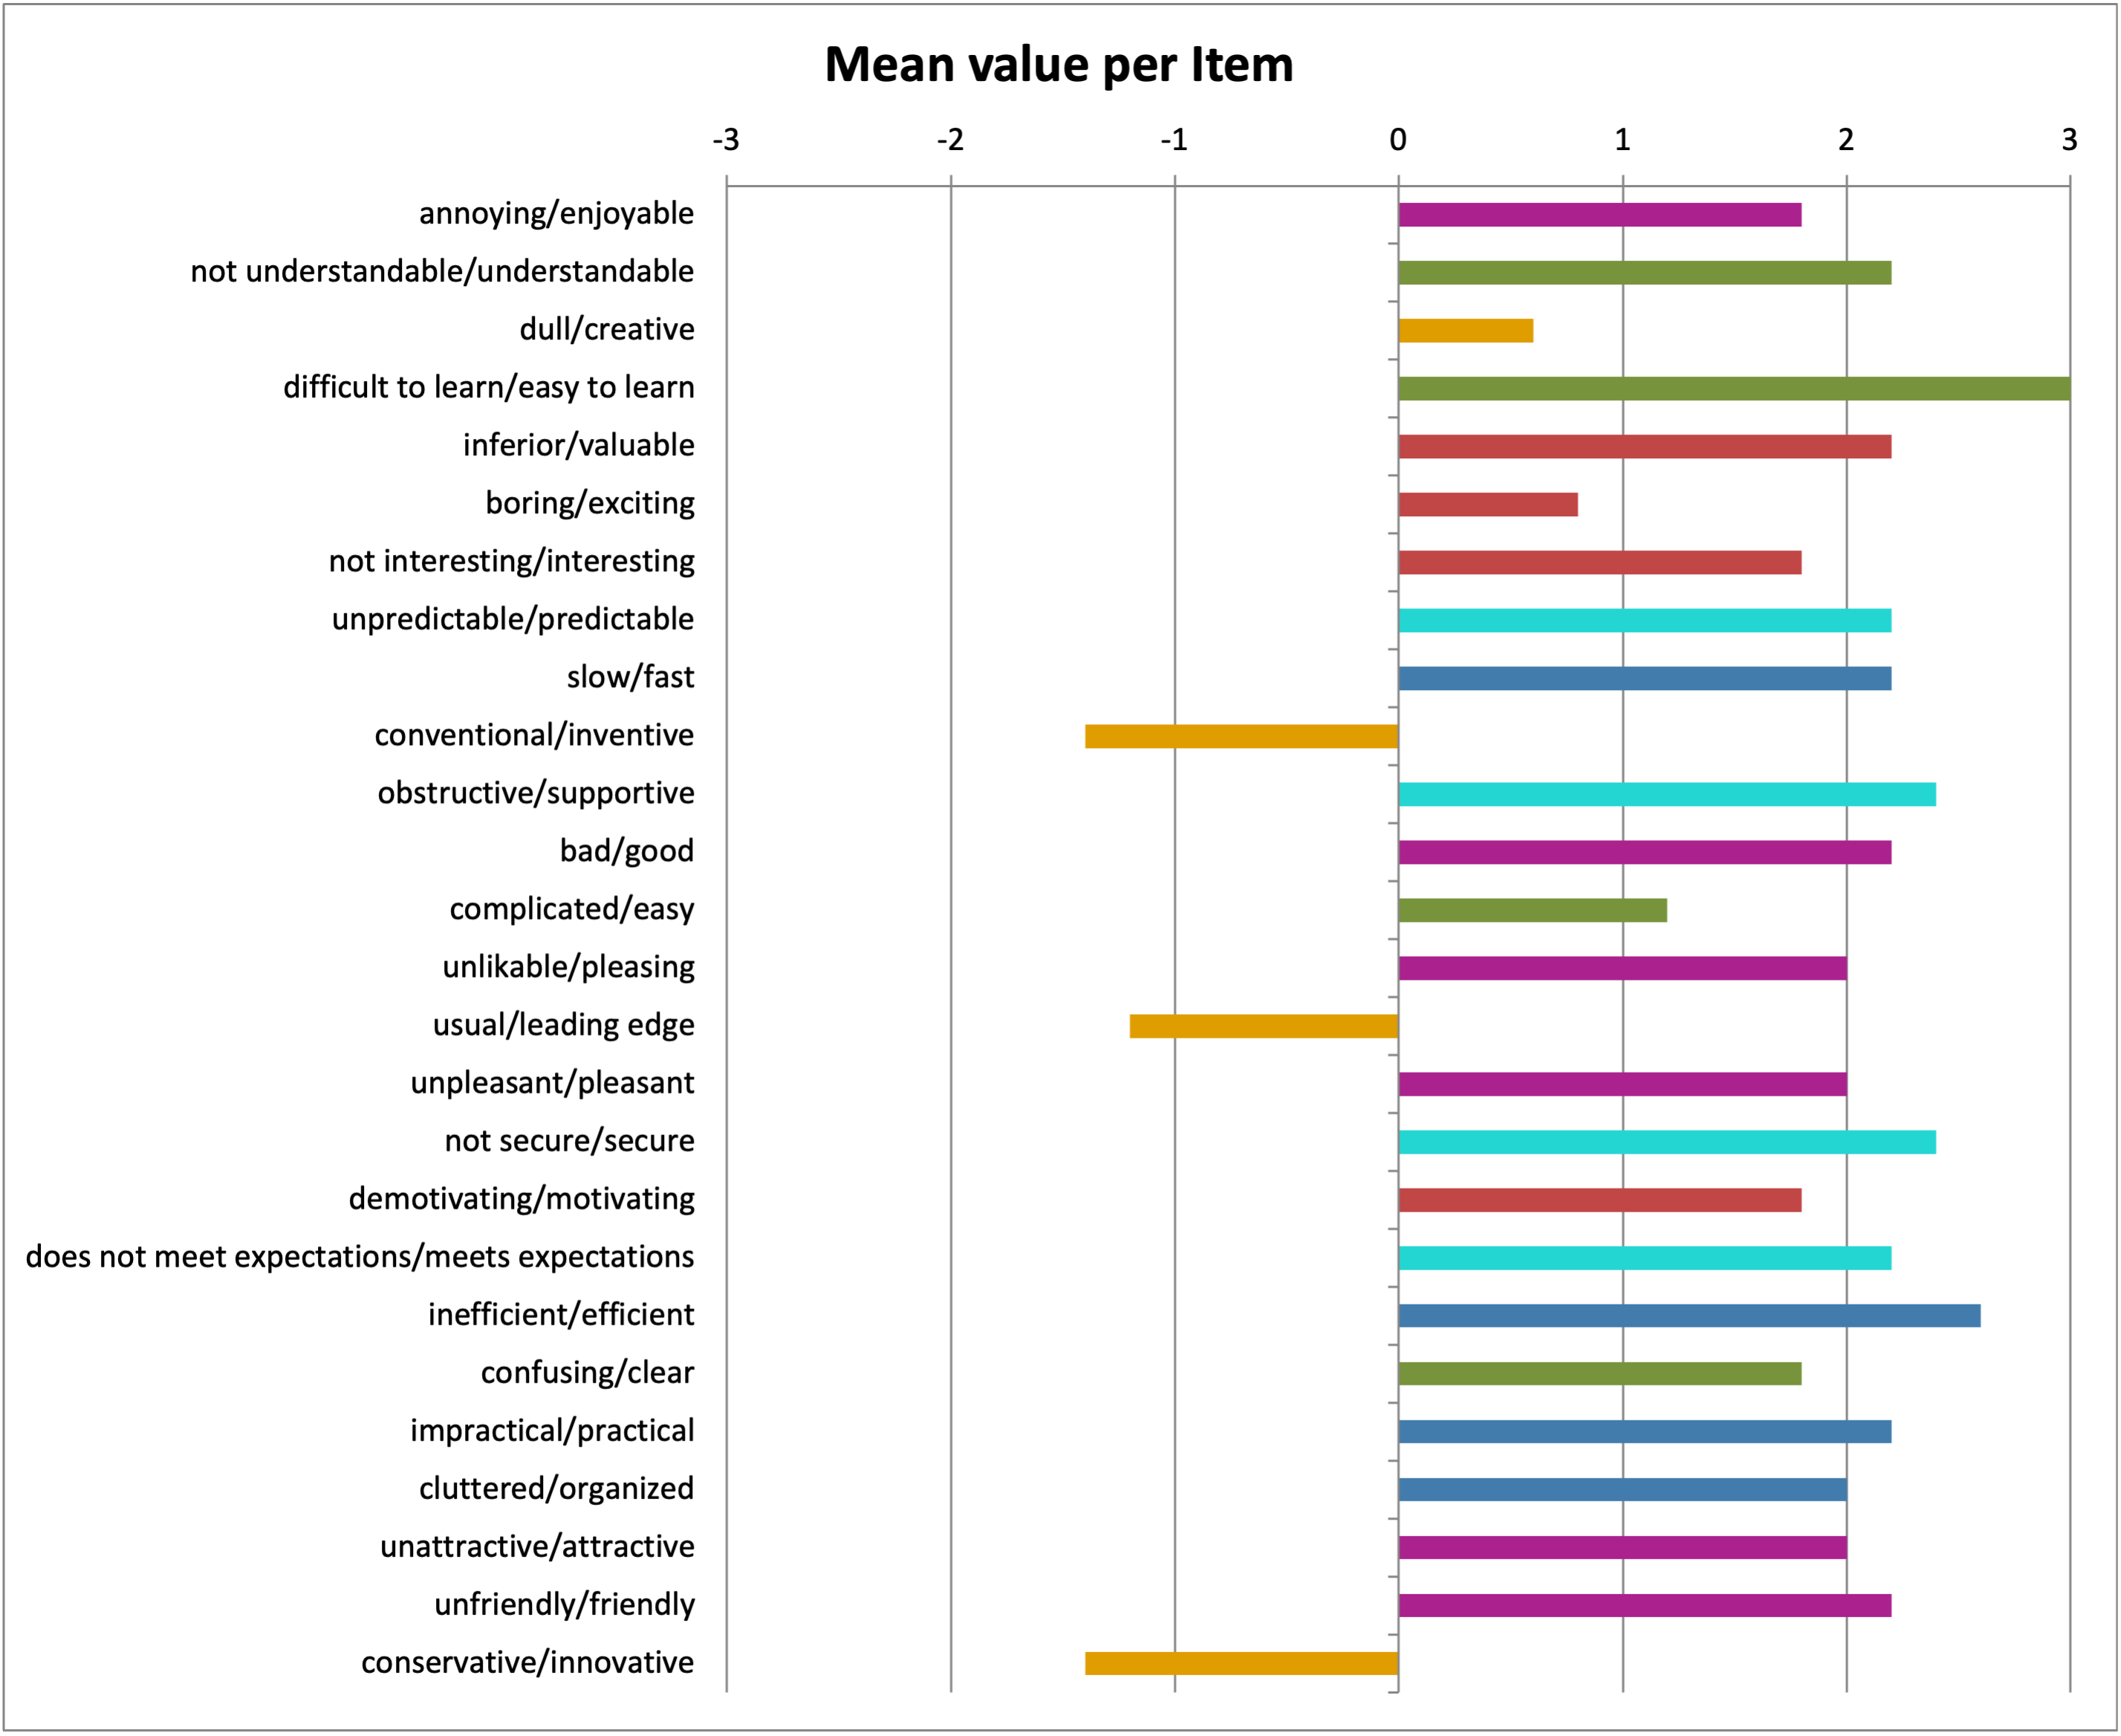
\includegraphics[width=150mm,scale=1]{./images/Result_Meanvalueperitem.png}}
                \caption{Mean value per item}
                \label{Mean value per item}
            \end{figure}

            Stimulation: The mean score for the stimulation scale is 1.7, indicating moderate stimulation, refer to Appendix A \tablename{ \ref{table:Mean value per item}}. Item 5 "valuable" received a relatively high score of 2.2, indicating perceived value. However, items 6 "boring" and 18 "demotivating" received low scores, suggesting unengaging aspects, refer to \figurename{\ref{Mean value per item}}.

            Dependability: The mean score for the dependability scale is 2.2, indicating relatively dependable. Items 8 "unpredictable", 11 "obstructive", and 19 "does not meet expectations" received scores below the mean, indicating issues with reliability or consistency , refer to Appendix A \tablename{ \ref{table:Mean value per item}}.

            Efficiency: The mean score for the efficiency scale is 2.2, indicating somewhat efficient, refer to Appendix A \tablename{ \ref{table:Mean value per item}}. Item 9 "fast" received a relatively high score of 2.2, indicating perceived speed. However, items 20 "inefficient", 22 "impractical", and 23 "cluttered" received scores below the mean, indicating usability and efficiency issues, refer to \figurename{\ref{Mean value per item}}.

            These UEQ results suggest that while the product was generally moderately attractive and dependable, there are issues with ease of use, innovation, and efficiency. Certain aspects of the product were also perceived as unengaging or demotivating. These insights can guide product designers and developers in identifying areas for improvement and prioritizing changes to improve user experience.
        
        
        %%%%%%%% UEQ Scales %%%%%%%
        \subsubsection{UEQ Scales}\hfill

            The study investigated the means, variances, and standard deviations of the ratings for each item, as well as the means and variances for each of the six UEQ scales: Attractiveness, Perspicuity, Efficiency, Dependability, Stimulation, and Novelty. The findings showed that the highest mean score was for Efficiency (2.250), followed by Dependability (2.300), and then Attractiveness and Perspicuity (both at 2.033 and 2.050, respectively). The lowest mean score was for Stimulation (1.650), and Novelty had a negative mean score (-0.850), indicating a lack of novelty in the product or service, refer to \figurename{\ref{UEQ Scales}} and Appendix A \tablename{ \ref{table: UEQ Scales}}.

            The variances for each scale indicated the amount of variation in the responses. Dependability had the highest variance (0.79), suggesting mixed experiences with the product or service's dependability, refer to Appendix A \tablename{ \ref{table: UEQ Scales}}. Novelty had the highest variance (1.18), indicating highly varied experiences with the product or service's novelty, refer to \figurename{\ref{UEQ Scales}}.

            Analyzing the individual items, Item 13 had the highest variance (2.4), implying highly varied experiences with the product or service's complexity. Item 10 had a negative mean score (-1.4), indicating that users did not find the product or service inventive, refer to Appendix A \tablename{ \ref{table: UEQ Scales}}. Item 26 also had a negative mean score (-1.4), implying that users did not find the product or service innovative, refer to Appendix A \tablename{ \ref{table: UEQ Scales}}.

            The results suggested that users found the product or service to be efficient and dependable but not stimulating or novel. There were mixed experiences with attractiveness and perspicuity.    
            
            \begin{figure}[H]
                \centering
                \begin{subfigure}[b]{0.45\textwidth}
                    \centerline{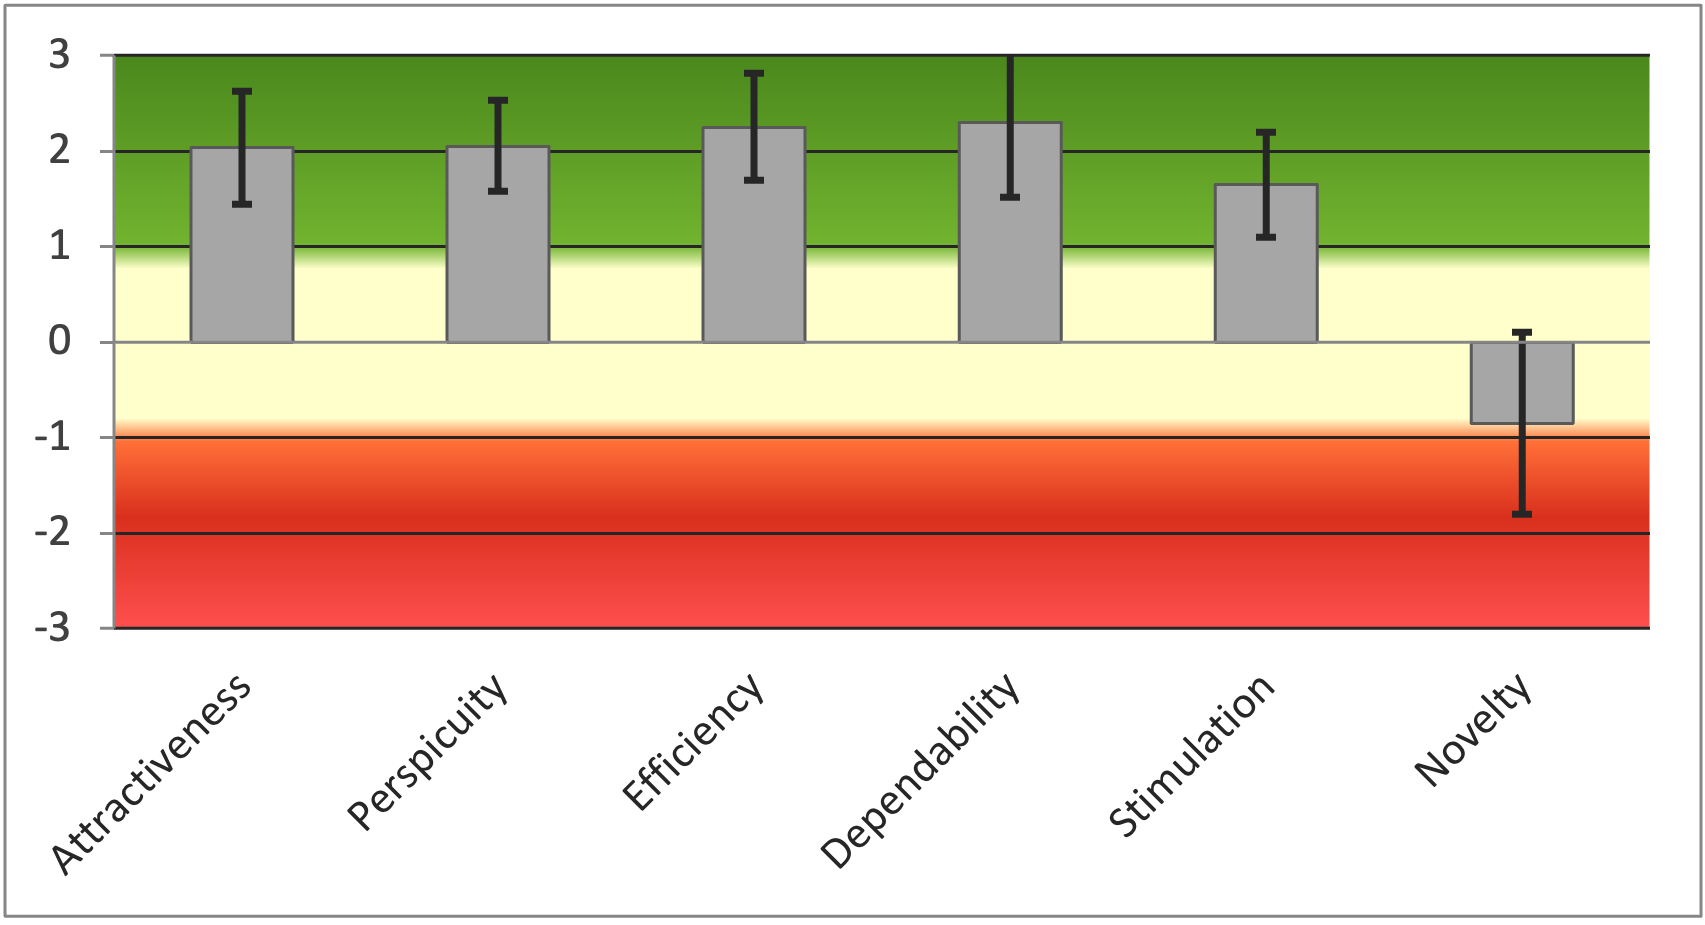
\includegraphics[width=80mm,scale=1]{./images/Resut_UEQ Scales.png}}
                    \caption{UEQ Scales}
                    \label{UEQ Scales}
                \end{subfigure}
                \hfill
                \begin{subfigure}[b]{0.45\textwidth}
                    \centerline{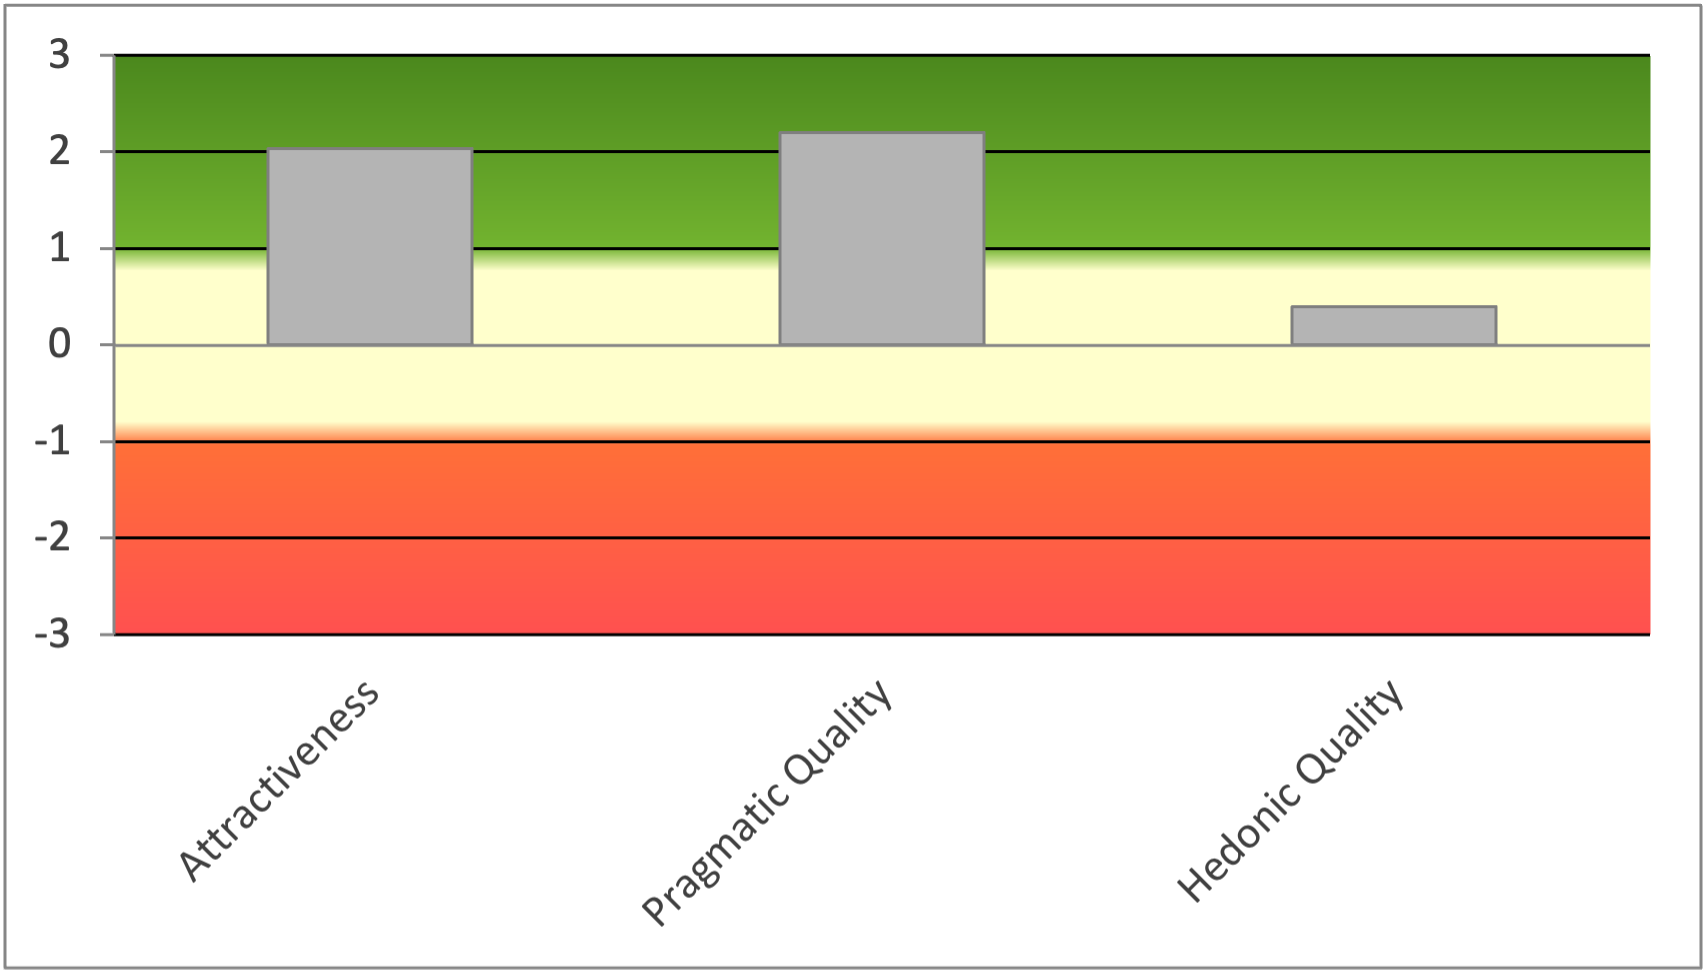
\includegraphics[width=80mm,scale=1]{./images/Results_Pragmatic and Hedonic Quality.png}}
                    \caption{Pragmatic and Hedonic Quality}
                    \label{Pragmatic and Hedonic Quality}
                \end{subfigure}
                \caption{Results UEQ Scales and Pragmatic \& Hedonic Quality}
                \label{fig:Results UEQ Scales and Pragmatic and Hedonic Quality}
            \end{figure}

        %%%%%%% Pragmatic and Hedonic Quality %%%%%%
        \subsubsection  {Pragmatic \& Hedonic Quality}\hfill
        
            Based on the UEQ pragmatic and hedonic quality dimensions, the overall attractiveness score of the user experience was 2.03, refer to Appendix A \tablename{ \ref{table: Pragmatic and Hedonic Quality}}. This score suggests that the participants rated the user experience slightly above average in terms of its overall attractiveness, refer to \figurename{\ref{Pragmatic and Hedonic Quality}}.

            The pragmatic quality score, which is a composite of Perspicuity (clarity), Efficiency, and Dependability, had a mean score of 2.20, refer to Appendix A \tablename{ \ref{table: Pragmatic and Hedonic Quality}}. This score indicates that the participants found the user experience to be slightly above average in terms of task-related quality aspects, refer to \figurename{\ref{Pragmatic and Hedonic Quality}}.

            The hedonic quality score, which is a composite of Stimulation and Novelty, had a mean score of 0.40. This score suggests that the participants found the user experience slightly below average in terms of non-task-related quality aspects, refer to Appendix A \tablename{ \ref{table: Pragmatic and Hedonic Quality}}.

            Of particular note is the negative mean score for Novelty (-0.85), which indicates that participants found the user experience less novel than expected, refer to \figurename{\ref{Pragmatic and Hedonic Quality}}.

            The results suggest that the user experience is generally perceived as slightly above average in terms of pragmatic quality, but slightly below average in terms of hedonic quality, with low scores specifically in terms of Novelty.

        %%%%%% Benchmark %%%%%%
        \subsubsection{Benchmark}\hfill

            Based on the benchmark results, the evaluated product has demonstrated impressive performance in terms of attractiveness, perspicuity, efficiency, and dependability, scoring among the top 10\% compared to other products. This indicates that users perceive the product as visually appealing, easy to understand, efficient to use, and reliable.

            However, the product's performance in terms of stimulation falls among the bottom 75\% of results, suggesting that users may not find the product very engaging or exciting, which could affect their overall satisfaction, refer to \figurename{\ref{UEQ Benchmark}}.

            Additionally, the product's novelty score is among the bottom 25\% of results, indicating that it may not be particularly innovative or unique compared to other products, refer to \figurename{\ref{UEQ Benchmark}}. While novelty may not be essential for all products, it can be crucial in highly competitive markets or products that require frequent updates to maintain user engagement.

            The benchmark shows that the evaluated product excels in pragmatic quality, but there is room for improvement in hedonic quality and novelty.
            
            \begin{figure}[H]
                \centering
                \begin{subfigure}[b]{0.6\textwidth}
                    \centerline{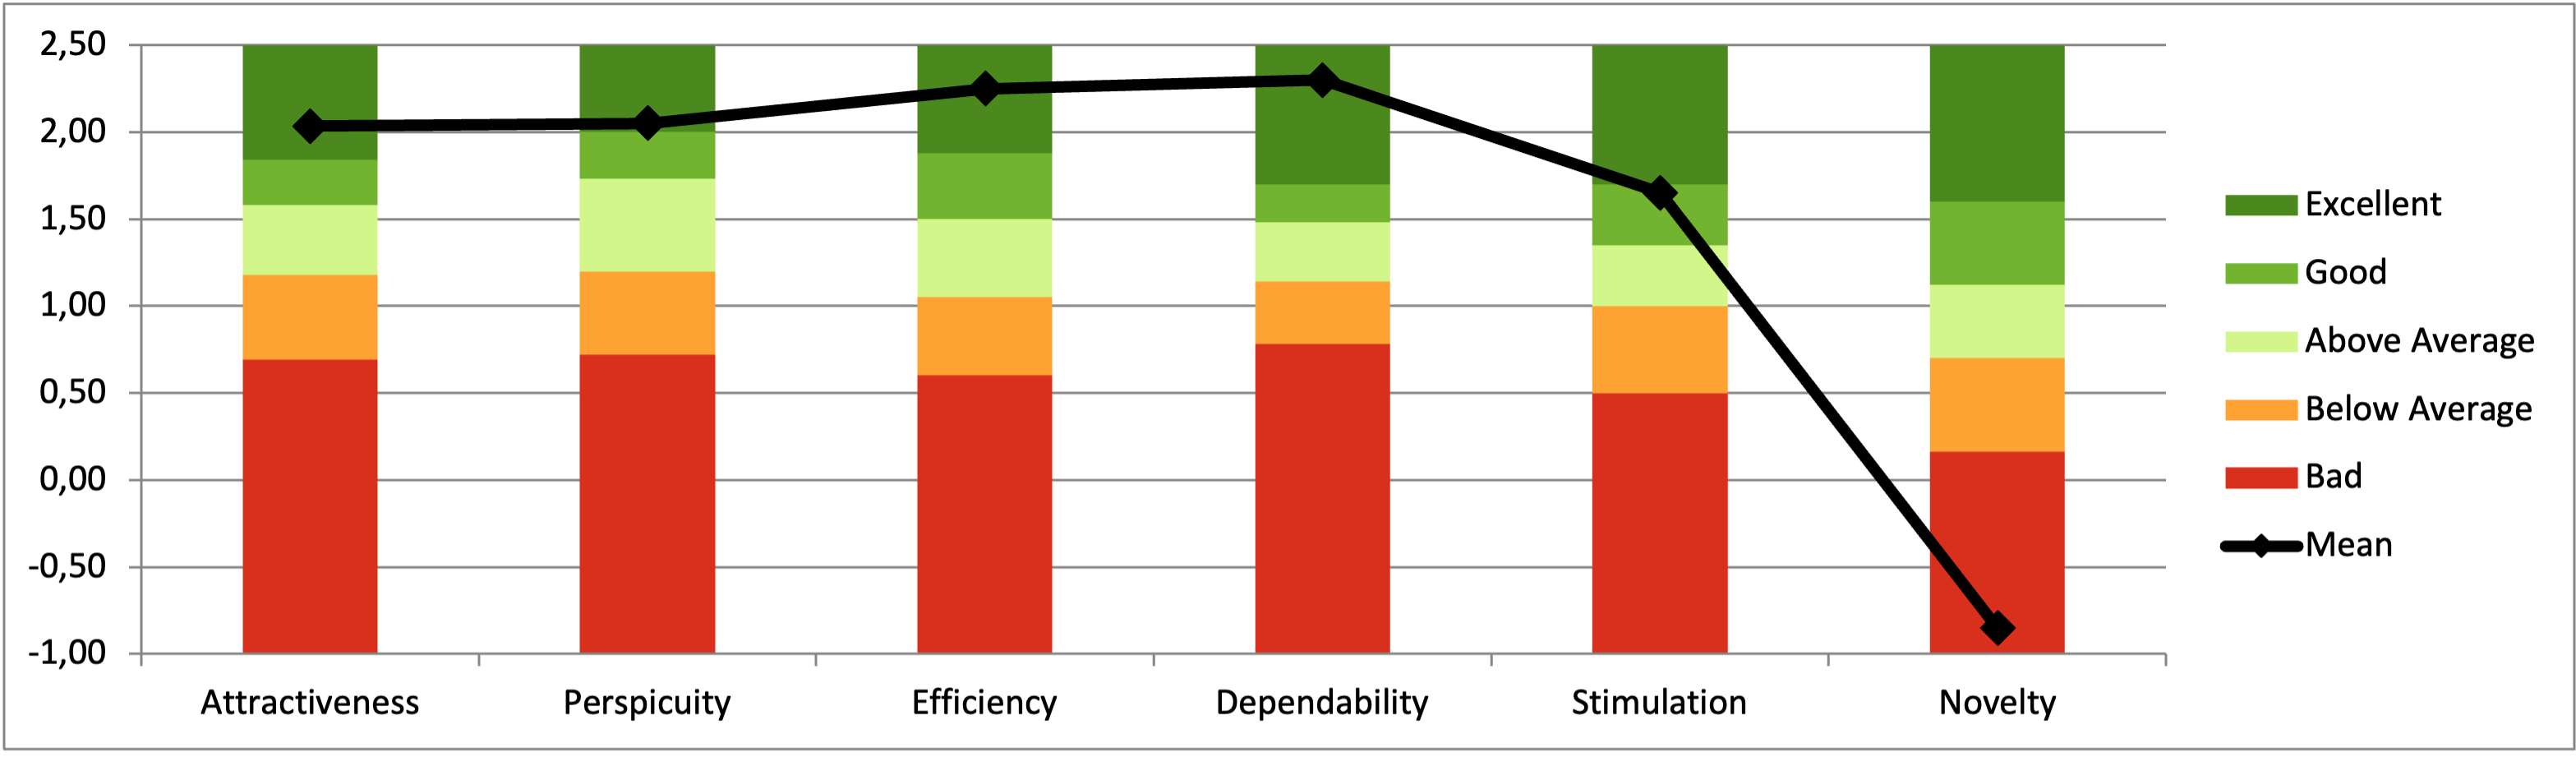
\includegraphics[height=35mm,scale=1]{./images/Resutls_Benchmark.png}}
                    \caption{UEQ Benchmark}
                    \label{UEQ Benchmark}
                \end{subfigure}
                \hfill
                \begin{subfigure}[b]{0.3\textwidth}
                    \centerline{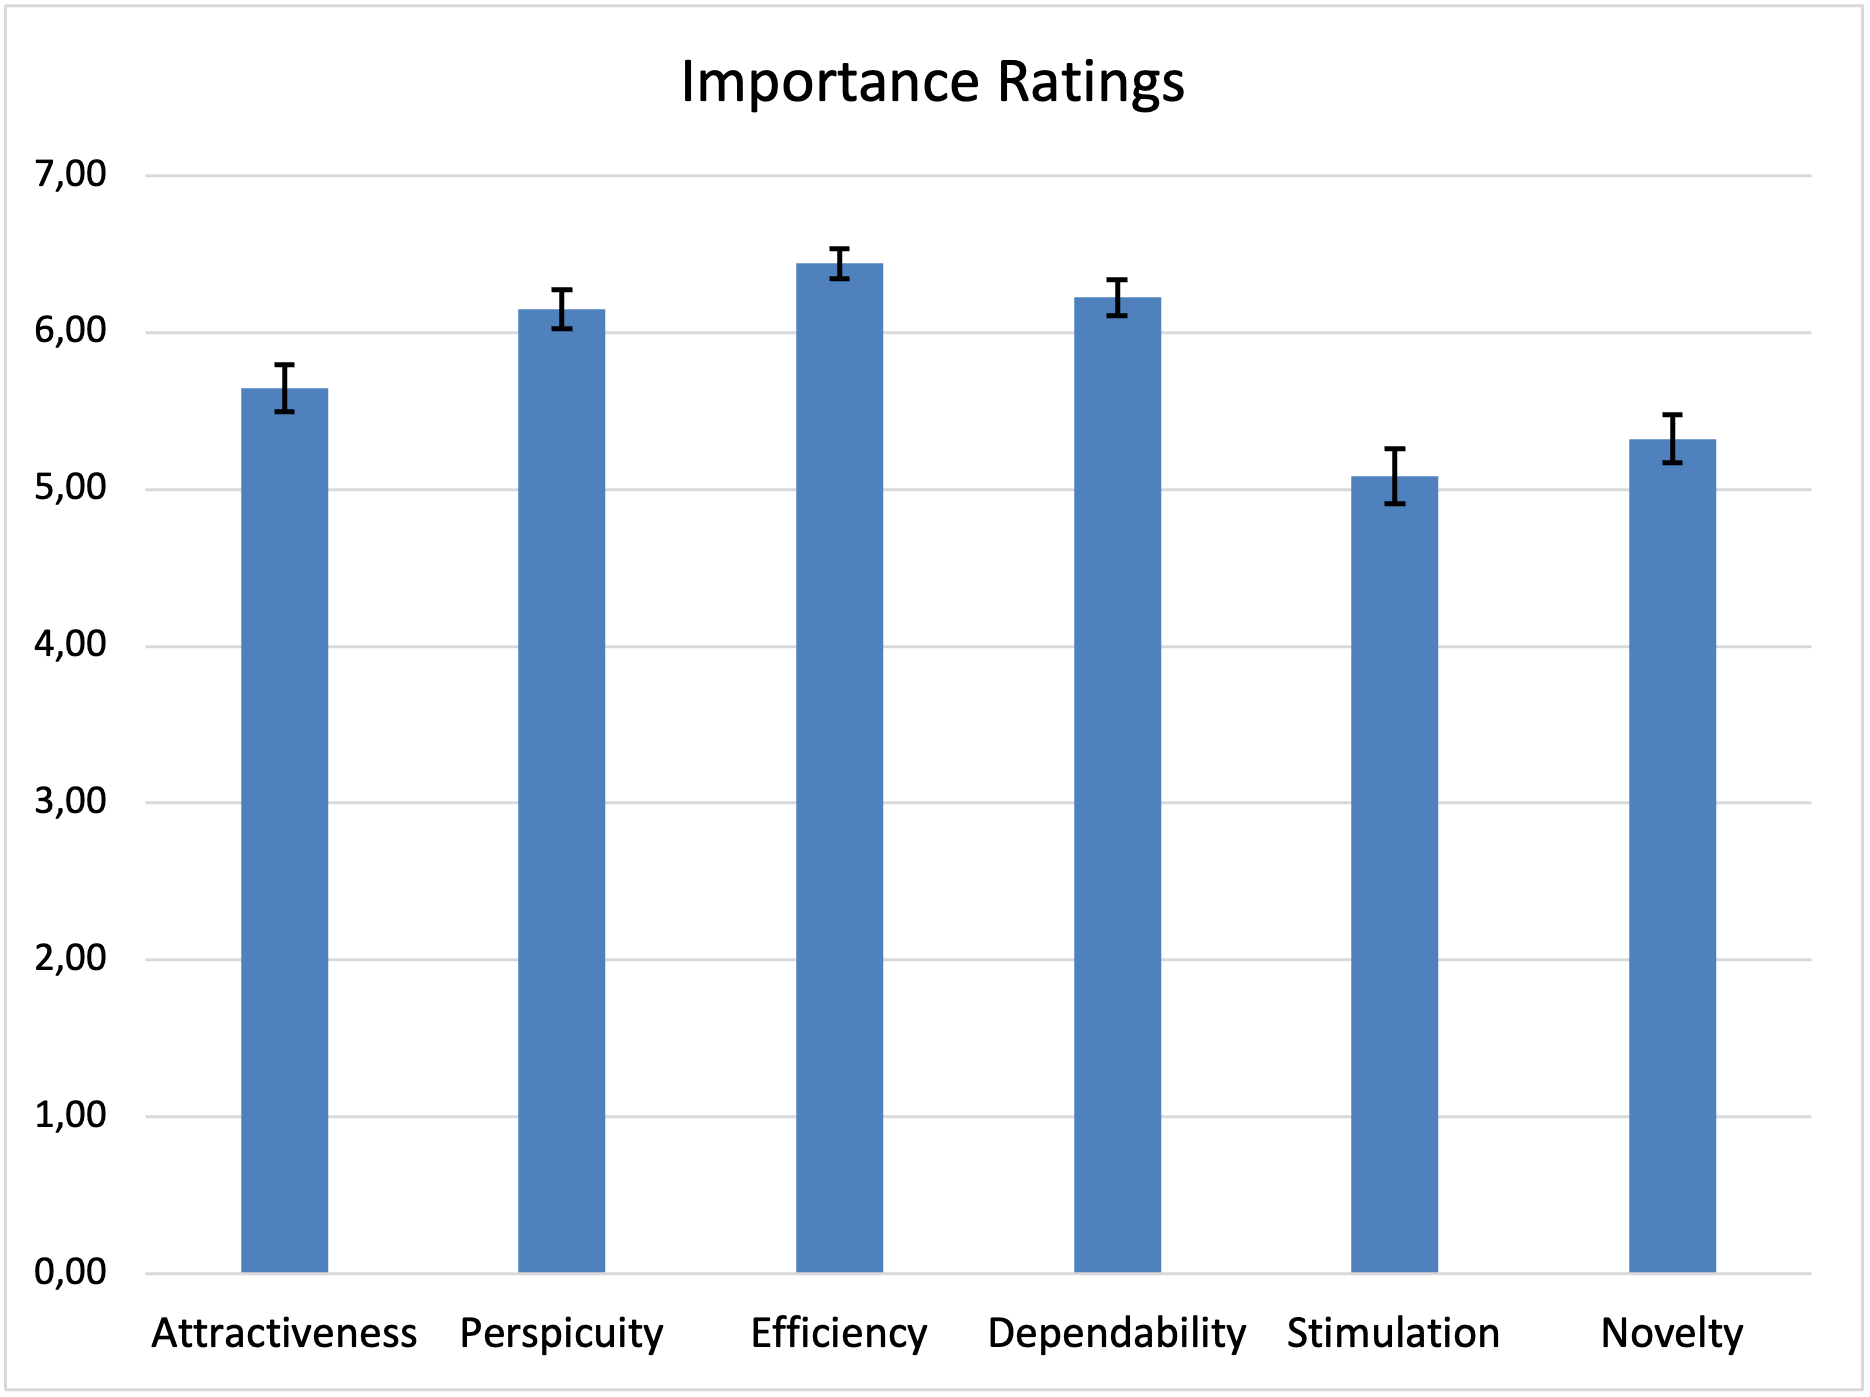
\includegraphics[height=40mm,scale=1]{./images/Results_KPUCalculation.png}}
                    \caption{KPI Calculation}
                    \label{KPI Calculation}
                \end{subfigure}
                \caption{Benchmark and KPI Calculation}
                \label{fig:Benchmark and KPI Calculation}
            \end{figure}
            %%%%%%%% KPI Calculation %%%%%%%%%%
            \subsubsection{KPI Calculation}\hfill

            The descriptive statistics of the UEQ scales, including mean, standard deviation, sample size, and confidence interval.

            To derive a Key Performance Indicator (KPI), a formula is necessary to combine the individual scale scores. A possible approach is to compute the arithmetic mean of all UEQ scale scores \cite{laugwitz2008construction}.

            With this formula, the resulting KPI is \cite{laugwitz2008construction}:

            KPI = (5.64 + 6.15 + 6.44 + 6.22 + 5.09 + 5.32) / 6 = 5.67, refer to \figurename{\ref{KPI Calculation}}

            This value represents the overall user experience score for the evaluated product, ranging from 0 to 8.

            The confidence intervals provide information about the precision of the estimated mean values. For instance, the attractiveness scale's estimated mean score is 5.64, with a 95\% confidence interval of [5.49, 5.79]. This indicates that there is a 95\% probability that the actual mean score of the population falls within this interval. Similarly, we can interpret the confidence intervals of the other UEQ scales.

        %%%%% Sample size %%%%%
        \subsubsection{Sample Size}\hfill

            \begin{table}[H]	
                \begin{center}
                    \begin{tabular}[H]{ |m{4cm}|m{2cm}|m{2cm}|m{2cm}|m{2cm}|m{2cm}|m{1cm}|}
                        \hline
                        \textbf{Condition}&\textbf{Attractiveness} &\textbf{Perspicuity} &\textbf{Efficiency}  &\textbf{Dependability}  &\textbf{Stimulation} &\textbf{Novelty}\\ \hline
                        Precision=0.5,Err.Prob.=0.1	    &5	    &3	    &4	    &9	    &4	    &13   \\ \hline  
                        Precision=0.5,Err.Prob.=0.05	&7	    &5	    &6	    &12	    &6	    &18   \\ \hline  
                        Precision=0.5,Err.Prob.=0.01	&12	    &8	    &11	    &21	    &10	    &31   \\ \hline  
                        Precision=0.25,Err.Prob.=0.1	&20	    &13	    &18	    &35	    &17	    &51   \\ \hline  
                        Precision=0.25,Err.Prob.=0.05	&28	    &18	    &25	    &49	    &24	    &72   \\ \hline  
                        Precision=0.25,Err.Prob.=0.01	&48	    &31	    &43	    &85	    &42	    &125  \\ \hline      
                        Precision=0.1,Err.Prob.=0.1	    &123	&80	    &111	&216	&107	&320  \\ \hline      
                        Precision=0.1,Err.Prob.=0.05	&173	&113	&156	&305	&151	&451  \\ \hline      
                        Precision=0.1,Err.Prob.=0.01	&300	&196	&270	&528	&262	&782  \\         
                        \hline
                    \end{tabular}
                \end{center}
                \caption{Sample Size}
                \label{Sample Size}
            \end{table}

            The present study has calculated various sample sizes for different levels of precision and error probability for each condition of the User Experience Questionnaire. The sample size estimation has been based on the assumption of a normal distribution with a standard deviation of 1, refer to \tablename{ \ref{Sample Size}}.

            For instance, taking the first row as an example, with a precision of 0.5 and an error probability of 0.1, the sample size for the Attractiveness condition is 5. This implies that to estimate the mean score for Attractiveness in this condition with a precision of 0.5 and an error probability of 0.1, researchers must have a sample size of at least 5, refer to \tablename{ \ref{Sample Size}}.

            Upon examining the table, we observe that the sample size increases as the precision and error probability become smaller. This trend occurs because higher precision and lower error probability require a larger amount of data to achieve statistical significance, refer to \tablename{ \ref{Sample Size}}.

            The \tablename{ \ref{Sample Size}} provides valuable insights for researchers interested in conducting studies utilizing the UEQ. By following these sample sizes as a guide, researchers can ensure that their studies have sufficient statistical power to detect meaningful differences between conditions.
        
\section{Discussion}

    The heuristic evaluation was conducted by an expert on three software applications developed by Delta3 Gmbh Software, namely the iOS delta3 app, the macOS application Editor, and the web-based operations portal. The evaluation identified a range of strengths and problems associated with each of the software applications. The observations demonstrate the importance of heuristic evaluation in identifying usability issues in software applications and guiding software developers and designers in making improvements that enhance the overall user experience and usability of the software.    Based on the UEQ benchmark results, the analyzed product has performed exceptionally well in all categories except for stimulation and novelty. Specifically, the attractiveness, perspicuity, efficiency, and dependability scales scored within the 10\% best results, indicating a high level of user satisfaction with the product in terms of these attributes. However, the stimulation scale had a good rating, indicating that 10\% of results were better, but 75\% of results were worse, suggesting that there is some room for improvement in terms of providing a more engaging and stimulating user experience. Additionally, the novelty scale had a bad rating, suggesting that the product's novelty score is in the range of the 25\% worst results. This indicates that the product may not be perceived as innovative or fresh by users, and there may be a need to introduce more novel and creative features to improve user experience.

    The study tested the usability of the Delta3 app/player with five participants of diverse backgrounds. Some completed tasks with ease, while others faced difficulties. Task 4 was the most difficult. Participants provided feedback on the app's strengths and problems, including issues with loading times, layout, and settings. The study's findings can be used to improve similar applications in the future.
    
    The UEQ KPI calculation provides a more detailed analysis of user experience by measuring mean scores, standard deviation, confidence intervals, and benchmark comparisons across all six UEQ scales. The results indicate that the product scored highest in the efficiency scale (mean=6.44), followed by the dependability scale (mean=6.22), and perspicuity scale (mean=6.15). These scores are all above the benchmark comparison, indicating that users were highly satisfied with these aspects of the product. The attractiveness scale had a mean score of 5.64, which is also above the benchmark comparison. However, this score had a relatively higher standard deviation (1.21), suggesting that user opinions were more diverse on this scale. The stimulation and novelty scales had lower mean scores of 5.09 and 5.32, respectively, which were also below the benchmark comparison. These results indicate that the product may need to improve in terms of providing a more stimulating and novel user experience.

    Lastly, the Cronbach's alpha coefficient analysis provides insights into the reliability of the UEQ measurement instrument used in the study. The alpha coefficient score of 0.86 indicates that the UEQ is highly reliable in measuring user experience across all six scales. The inter-item correlations suggest that the items in each scale are positively correlated, indicating that they measure the same underlying construct. However, some items in the perspicuity and efficiency scales have a "DIV/0!" value, which could affect the reliability of these scales. The analysis also provides a confidence interval for the alpha coefficient, indicating that the true reliability of the instrument falls between 0.21 and 0.98 at a 5\% level of significance.

    Based on the analysis of the software usability results, it can be concluded that overall, the software has moderate usability, with an average UEQ score of 0.51. The highest rated aspect of usability was "Dependability" with a score of 0.76, while the lowest rated aspect was "Novelty" with a score of 0.31. The Cronbach's alpha coefficient for the UEQ was 0.86, indicating a high level of internal consistency.

    However, it is important to note that the sample size for the UEQ was relatively small, with only 5 participants. This may limit the generalizability of the results and larger sample sizes should be considered in future usability testing.

    Overall, the results suggest that while the software has some usability issues, it is generally acceptable for use. Further improvements could be made in the areas of stimulation and novelty to enhance user engagement and satisfaction.

\section{Conclusion}
    In conclusion, the heuristic evaluation and UEQ benchmark results indicate that the Delta3 software applications have both strengths and weaknesses in terms of usability and user experience. While the software scored highly in terms of efficiency, dependability, and perspicuity, there is room for improvement in terms of providing a more stimulating and novel user experience. The study's findings suggest that the software has moderate usability, with an average UEQ score of 0.51. The Cronbach's alpha coefficient analysis indicates a high level of internal consistency, but the small sample size of the UEQ may limit the generalizability of the results. Overall, the study highlights the importance of usability testing and user experience evaluation in improving software design and enhancing the overall user experience.
% use section* for acknowledgment
\section*{Acknowledgment}
	I sincerely appreciate the help and guidance received from Prof. Dr. Dr. Dr. Carsten Roöcker. I would especially want to thank Mario Heinz-Jakobs, M.Sc., for his continued assistance whenever it was required, and I would also like to express my sincere gratitude to all survey respondents who gave me the insightful feedback.

\newpage
\section*{Appendix}

    \begin{table}[H]	
        \begin{center}
            \begin{tabular}[H]{ |m{1cm}|m{1cm}|m{1cm}|m{1cm}|m{1cm}|m{3cm}|m{3cm}|m{3cm}|}
                \hline
                \textbf{Item}&\textbf{Mean} &\textbf{Variance} &\textbf{Std. Dev.}  &\textbf{No.}  &\textbf{Left} &\textbf{Right} &\textbf{Scale}\\ \hline
                1	&1,8	&0,2	&0,4	&5	&annoying	            &enjoyable	                &Attractiveness             \\ \hline
                2	&2,2	&0,2	&0,4	&5	&not                    &understandable	            &understandable	Perspicuity         \\ \hline
                3	&0,6	&2,3	&1,5	&5	&creative	            &dull	                    &Novelty        \\ \hline
                4	&3,0	&0,0	&0,0	&5	&easy to learn	        &difficult to learn	        &Perspicuity        \\ \hline
                5	&2,2	&0,2	&0,4	&5	&valuable	            &inferior	                &Stimulation        \\ \hline
                6	&0,8	&1,7	&1,3	&5	&boring	                &exciting	                &Stimulation        \\ \hline
                7	&1,8	&0,7	&0,8	&5	&not interesting	    &interesting	            &Stimulation        \\ \hline
                8	&2,2	&1,2	&1,1	&5	&unpredictable	        &predictable	            &Dependability      \\ \hline
                9	&2,2	&1,7	&1,3	&5	&fast	                &slow	                    &Efficiency     \\ \hline
                10	&-1,4	&2,3	&1,5	&5	&inventive	            &conventional	            &Novelty        \\ \hline
                11	&2,4	&0,3	&0,5	&5	&obstructive	        &supportive	                &Dependability      \\ \hline
                12	&2,2	&0,7	&0,8	&5	&good	                &bad	                    &Attractiveness     \\ \hline
                13	&1,2	&5,7	&2,4	&5	&complicated	        &easy	                    &Perspicuity        \\ \hline
                14	&2,0	&1,0	&1,0	&5	&unlikable	            &pleasing	                &Attractiveness     \\ \hline
                15	&-1,2	&2,7	&1,6	&5	&usual	                &leading edge	            &Novelty        \\ \hline
                16	&2,0	&0,5	&0,7	&5	&unpleasant	            &pleasant	                &Attractiveness     \\ \hline
                17	&2,4	&0,8	&0,9	&5	&secure	                &not secure	                &Dependability      \\ \hline
                18	&1,8	&0,2	&0,4	&5	&motivating	            &demotivating	            &Stimulation        \\ \hline
                19	&2,2	&1,7	&1,3	&5	&meets expectations     &does not meet expectations	&Dependability      \\ \hline
                20	&2,6	&0,3	&0,5	&5	&inefficient	        &efficient	                &Efficiency     \\ \hline
                21	&1,8	&0,7	&0,8	&5	&clear	                &confusing	                &Perspicuity        \\ \hline
                22	&2,2	&0,7	&0,8	&5	&impractical	        &practical	                &Efficiency     \\ \hline
                23	&2,0	&1,0	&1,0	&5	&organized	            &cluttered	                &Efficiency     \\ \hline
                24	&2,0	&1,5	&1,2	&5	&attractive	            &unattractive	            &Attractiveness     \\ \hline
                25	&2,2	&0,7	&0,8	&5	&friendly	            &unfriendly	                &Attractiveness     \\ \hline
                26	&-1,4	&2,3	&1,5	&5	&conservative	        &innovative	                &Novelty        \\ 
                \hline
            \end{tabular}
        \end{center}
        \caption{Mean value per item}
        \label{table:Mean value per item}
    \end{table}

    \begin{table}[H]	
        \begin{center}
            \begin{tabular}[H]{ |c|c|c|}
                \hline
                \multicolumn{3}{|c|}{\textbf{UEQ Scales (Mean and Variance)}}\\
                \hline
                Attractiveness	&2,033	&0,45 \\ \hline
                Perspicuity	    &2,050	&0,29 \\ \hline
                Efficiency	    &2,250	&0,41 \\ \hline
                Dependability	&2,300	&0,79 \\ \hline
                Stimulation	    &1,650	&0,39 \\ \hline
                Novelty	        &-0,850	&1,18 \\
                \hline
            \end{tabular}
        \end{center}
        \caption{UEQ Scales}
        \label{table: UEQ Scales}
    \end{table}

    \begin{table}[H]	
        \begin{center}
            \begin{tabular}[H]{ |c|c|}
                \hline
                \multicolumn{2}{|c|}{\textbf{Pragmatic and Hedonic Quality)}} \\
                \hline
                Attractiveness	    &2,03 \\ \hline
                Pragmatic Quality	&2,20 \\ \hline
                Hedonic Quality	    &0,40 \\
                \hline
            \end{tabular}
        \end{center}
        \caption{Pragmatic and Hedonic Quality}
        \label{table: Pragmatic and Hedonic Quality}
    \end{table}

    \begin{figure}[H]
        \centerline{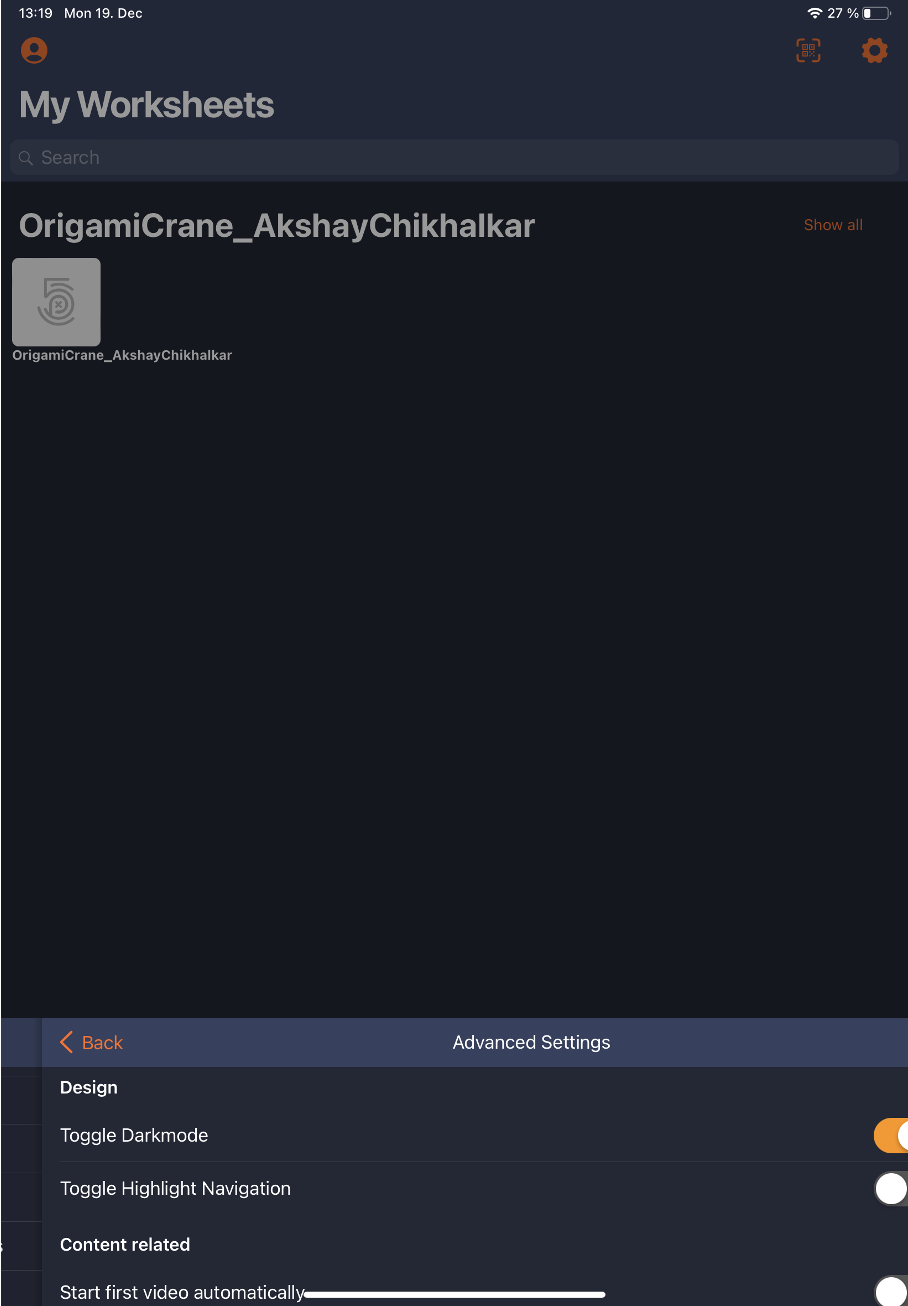
\includegraphics[width=80mm,scale=1]{./images/App_Strength_1.png}}
        \caption{App Strength 1}
        \label{App Strength 1}
    \end{figure}
    \begin{figure}[H]
        \centerline{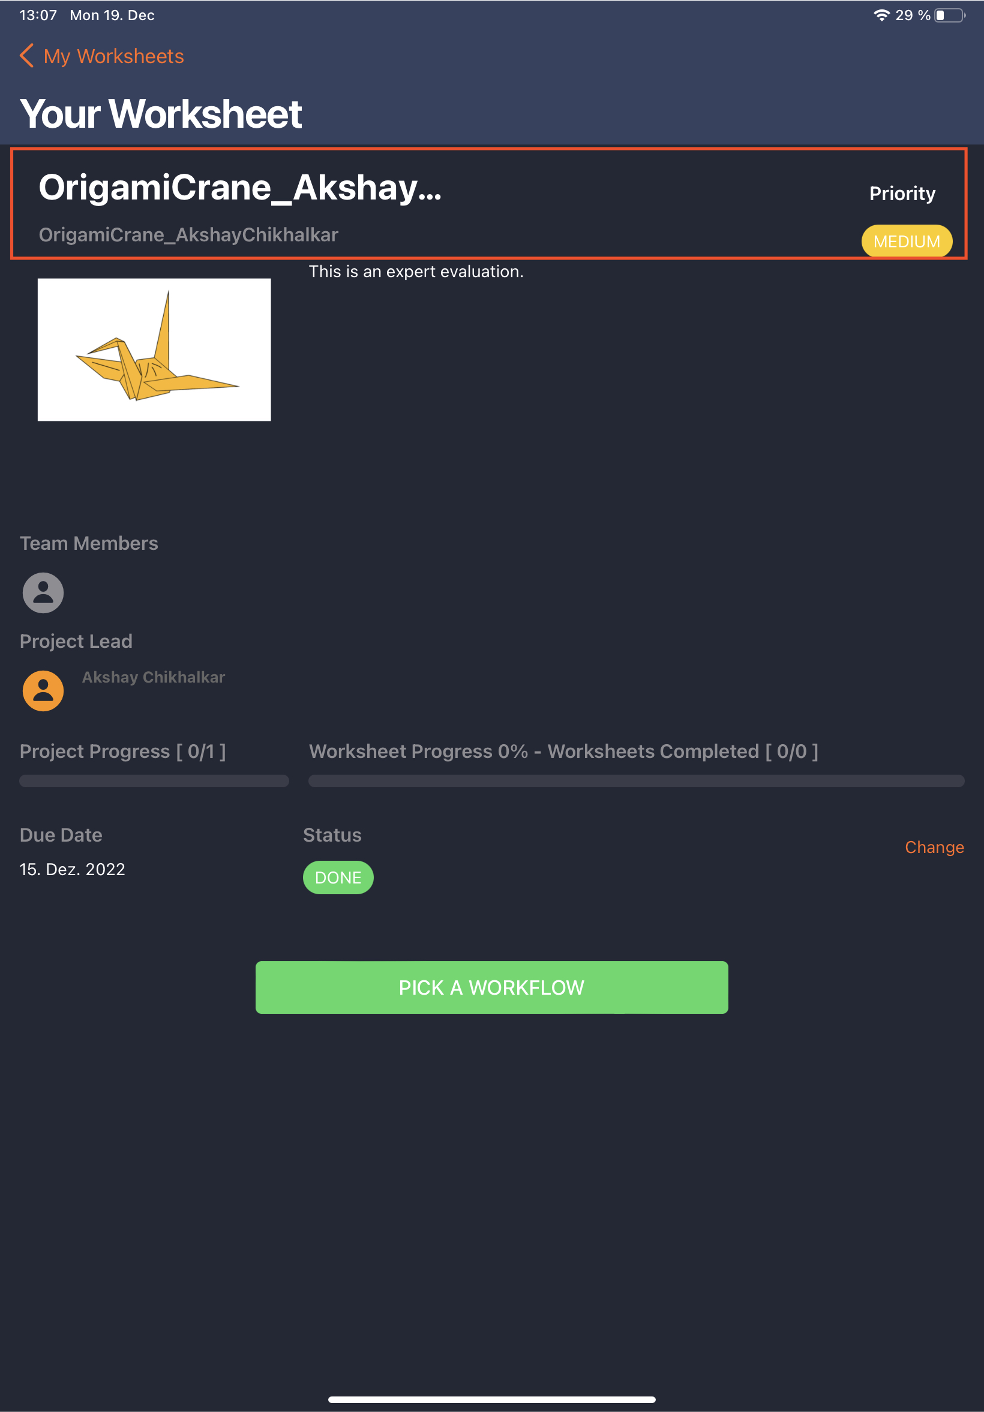
\includegraphics[width=75mm,scale=1]{./images/App_Problem_1.png}}
        \caption{App Problem 1}
        \label{App Problem 1}
    \end{figure}
    \begin{figure}[H]
        \centerline{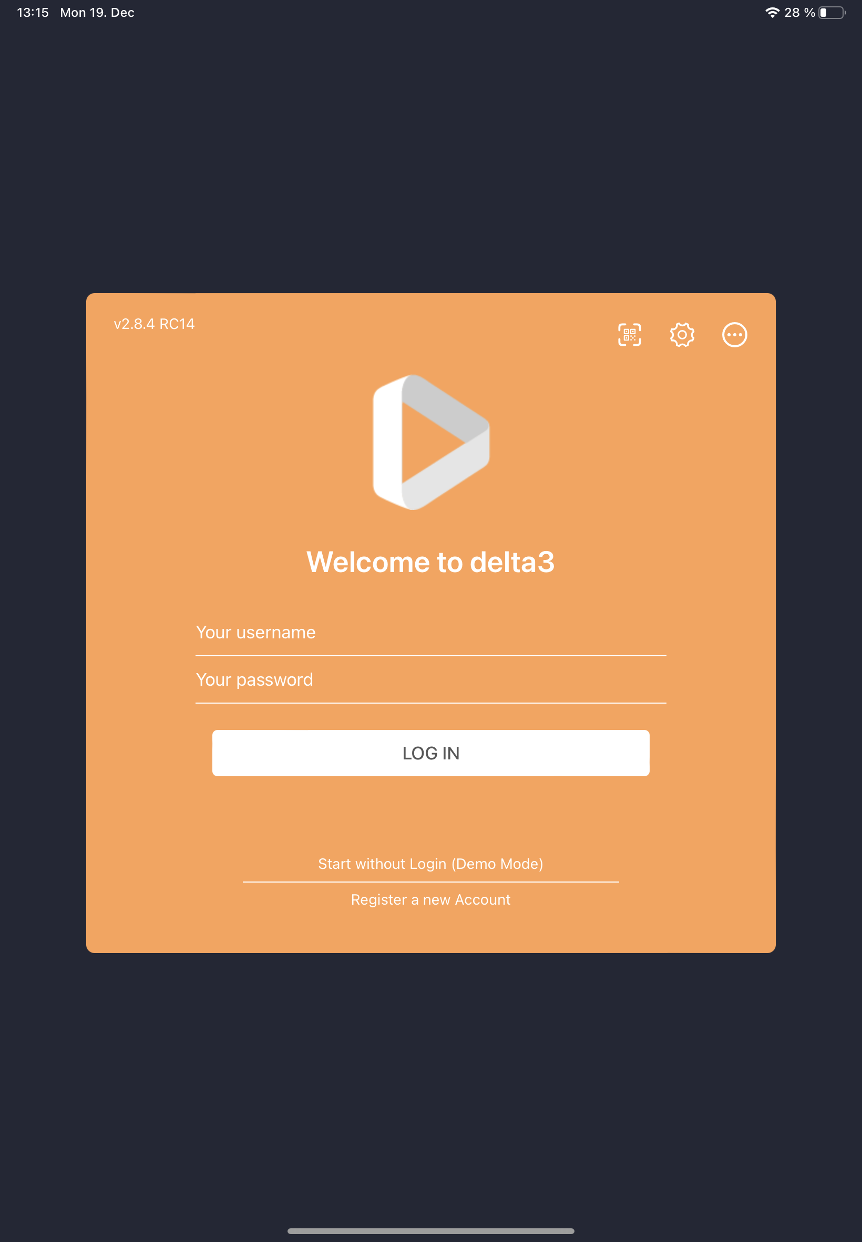
\includegraphics[width=75mm,scale=1]{./images/App_Problem_2.png}}
        \caption{App Problem 2}
        \label{App Problem 2}
    \end{figure}
    \begin{figure}[H]
        \centerline{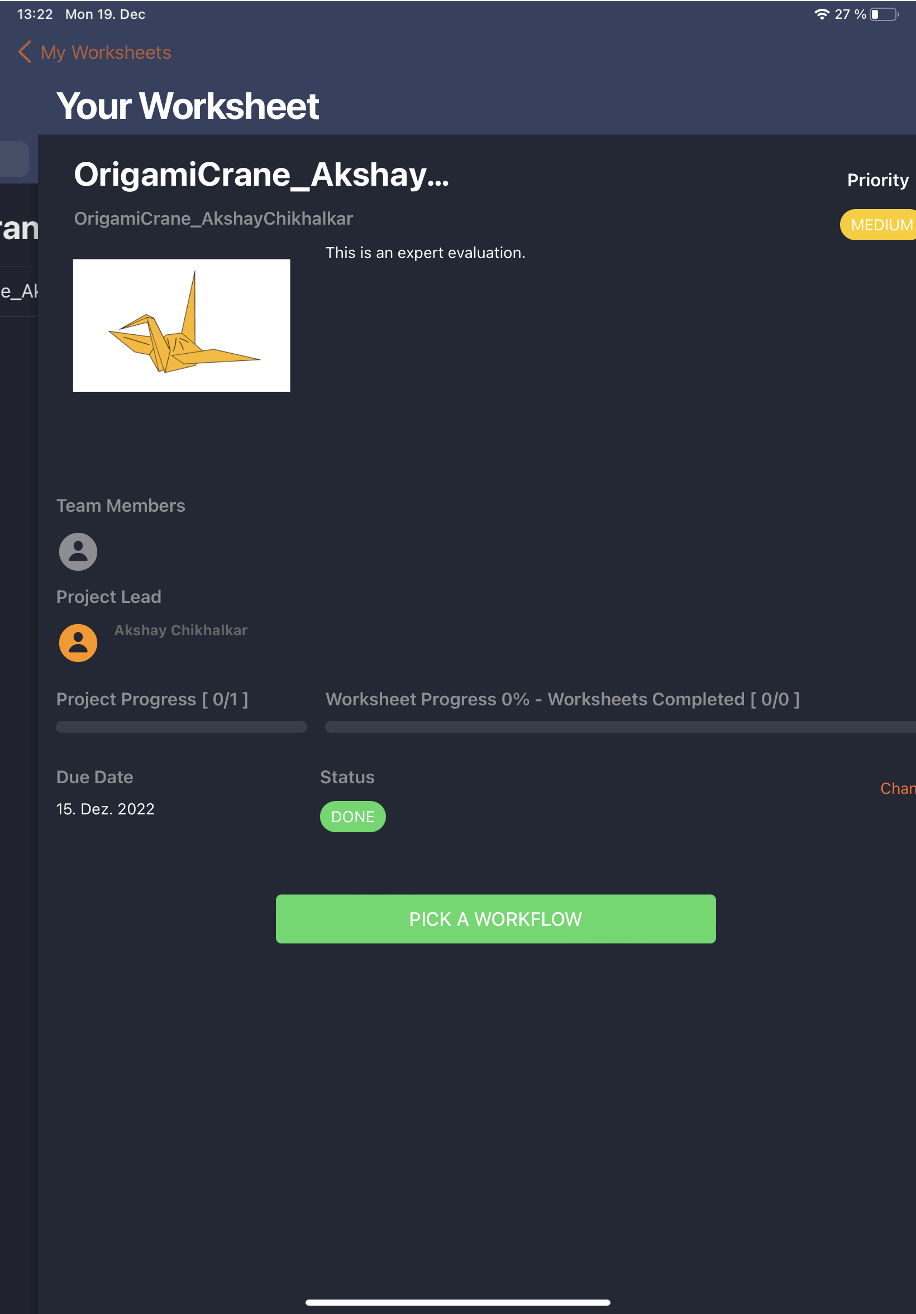
\includegraphics[width=75mm,scale=1]{./images/App_Problem_3.png}}
        \caption{App Problem 3}
        \label{App Problem 3}
    \end{figure}
    \begin{figure}[H]
        \centerline{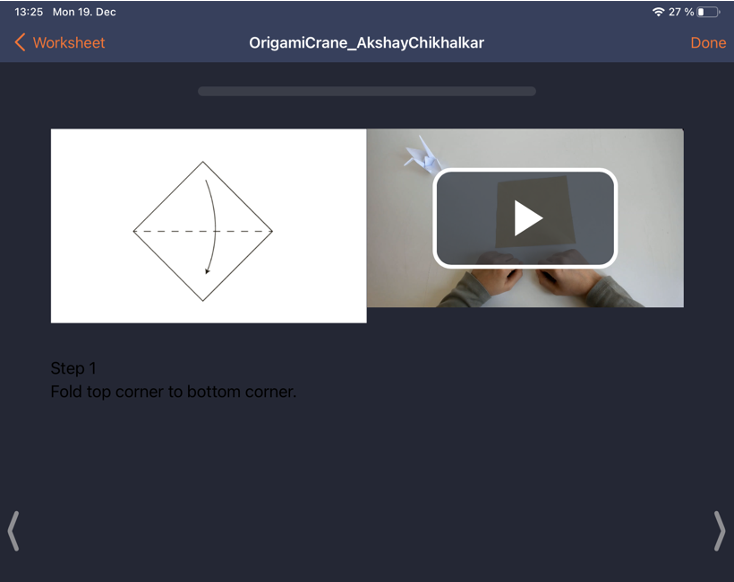
\includegraphics[width=100mm,scale=1]{./images/App_Problem_4.png}}
        \caption{App Problem 4}
        \label{App Problem 4}
    \end{figure}
    \begin{figure}[H]
        \centerline{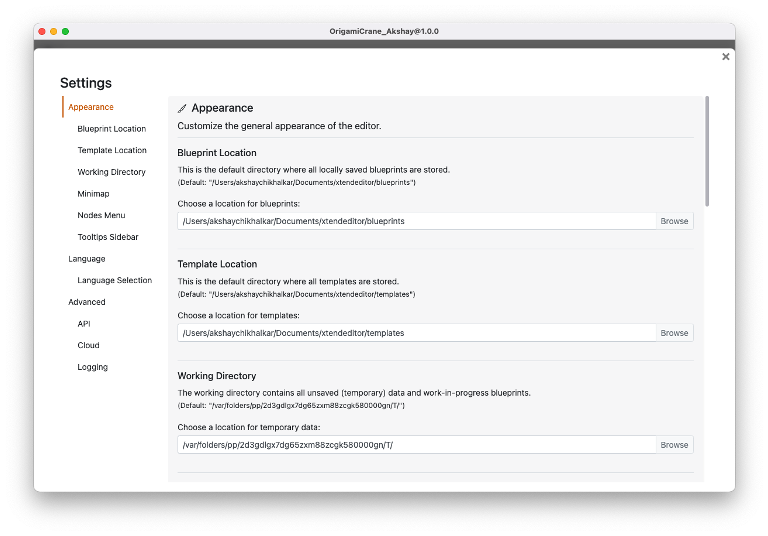
\includegraphics[width=100mm,scale=1]{./images/Editor_Strength_1.png}}
        \caption{Editor Strength 1}
        \label{Editor Strength 1}
    \end{figure}
    \begin{figure}[H]
        \centerline{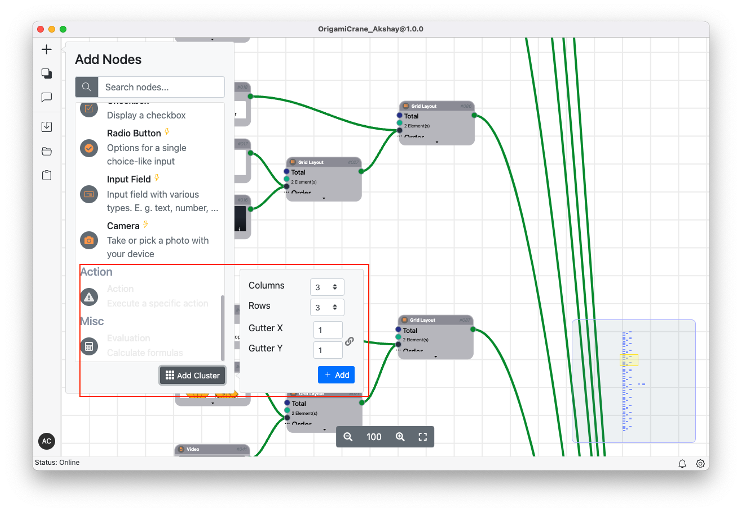
\includegraphics[width=100mm,scale=1]{./images/Editor_Strength_2.png}}
        \caption{Editor Strength 2}
        \label{Editor Strength 2}
    \end{figure}
    \begin{figure}[H]
        \centerline{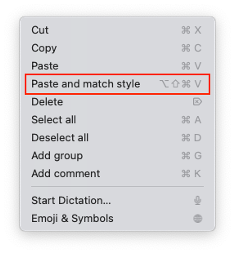
\includegraphics[height=50mm,scale=1]{./images/Editor_Strength_3.png}}
        \caption{Editor Strength 3}
        \label{Editor Strength 3}
    \end{figure}
    \begin{figure}[H]
        \centerline{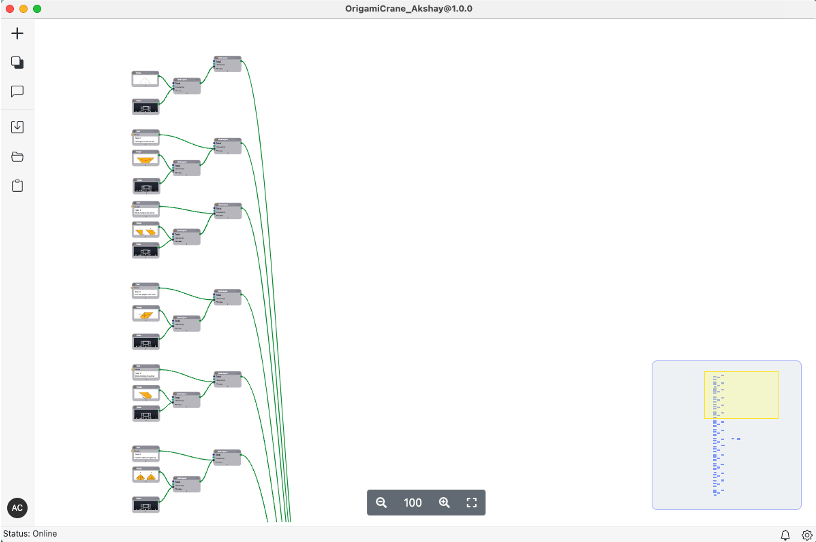
\includegraphics[width=100mm,scale=1]{./images/Editor_Problem_1.png}}
        \caption{Editor Problem 1}
        \label{Editor Problem 1}
    \end{figure}   
    \begin{figure}[H]
        \centerline{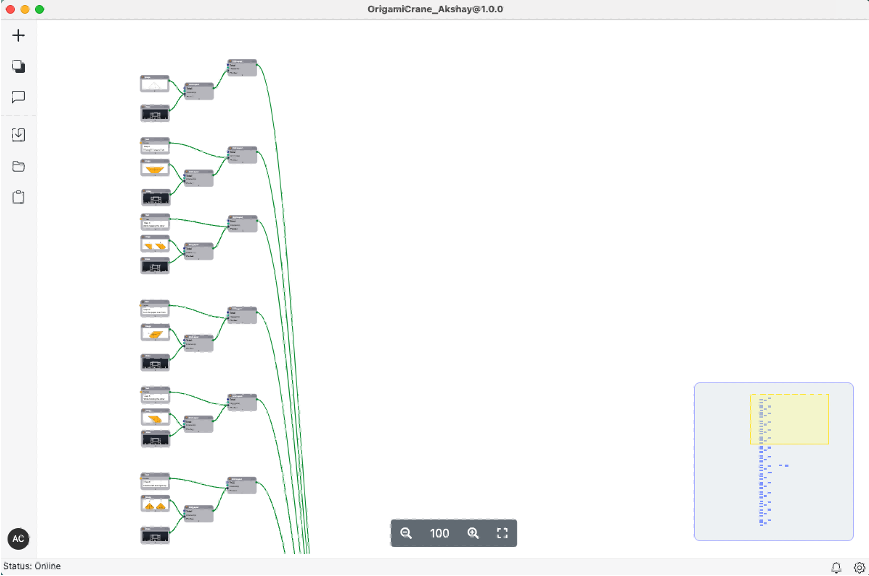
\includegraphics[width=100mm,scale=1]{./images/Editor_Problem_2.png}}
        \caption{Editor Problem 2}
        \label{Editor Problem 2}
    \end{figure}   
    \begin{figure}[H]
        \centerline{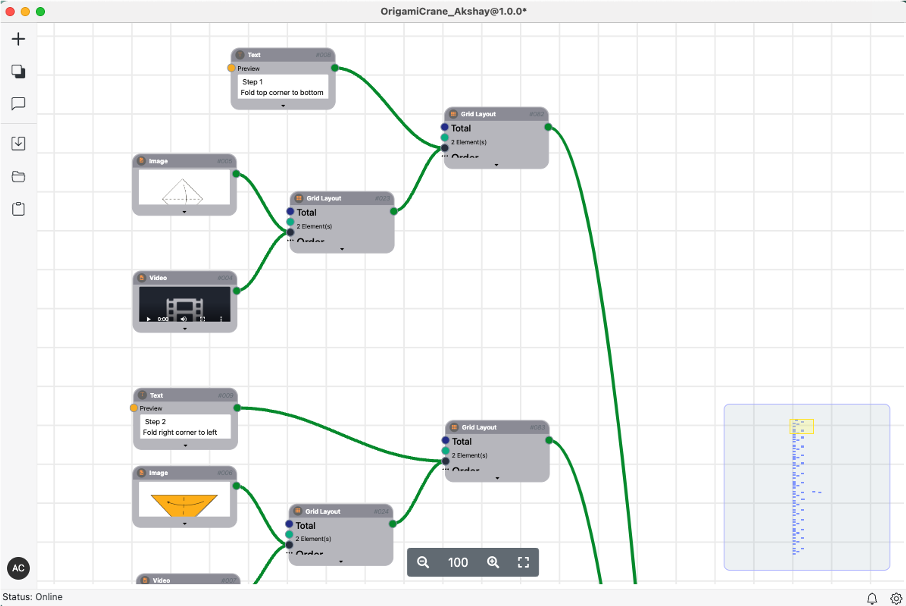
\includegraphics[width=100mm,scale=1]{./images/Editor_Problem_3.png}}
        \caption{Editor Problem 3}
        \label{Editor Problem 3}
    \end{figure}   
    \begin{figure}[H]
        \centerline{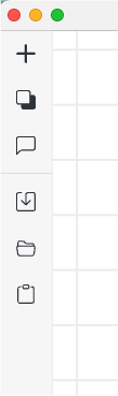
\includegraphics[height=50mm,scale=1]{./images/Editor_Problem_4.png}}
        \caption{Editor Problem 4}
        \label{Editor Problem 4}
    \end{figure}   
    \begin{figure}[H]
        \centerline{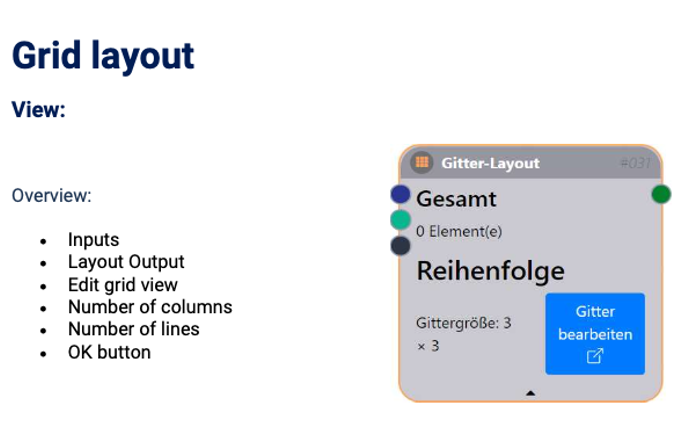
\includegraphics[width=100mm,scale=1]{./images/Editor_Problem_5.png}}
        \caption{Editor Problem 5}
        \label{Editor Problem 5}
    \end{figure}   
    \begin{figure}[H]
        \centerline{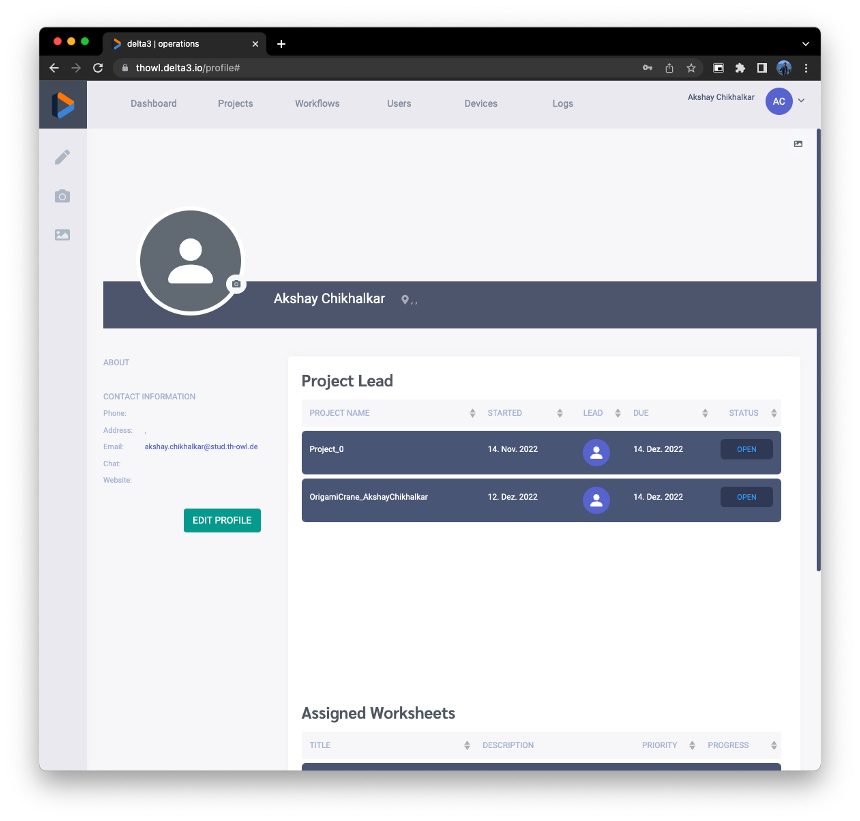
\includegraphics[width=100mm,scale=1]{./images/Operation_Strength_1.png}}
        \caption{Operation Strength 1}
        \label{Operation Strength 1}
    \end{figure}  
    \begin{figure}[H]
        \centerline{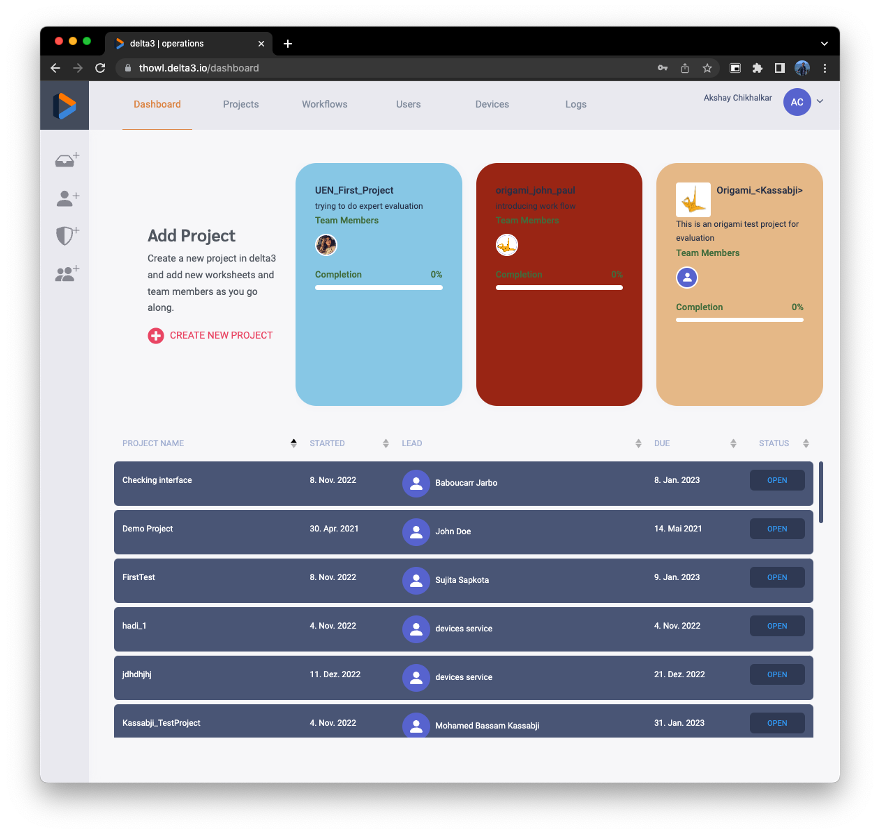
\includegraphics[width=100mm,scale=1]{./images/Operation_Strength_2.png}}
        \caption{Operation Strength 2}
        \label{Operation Strength 2}
    \end{figure}  
    \begin{figure}[H]
        \centerline{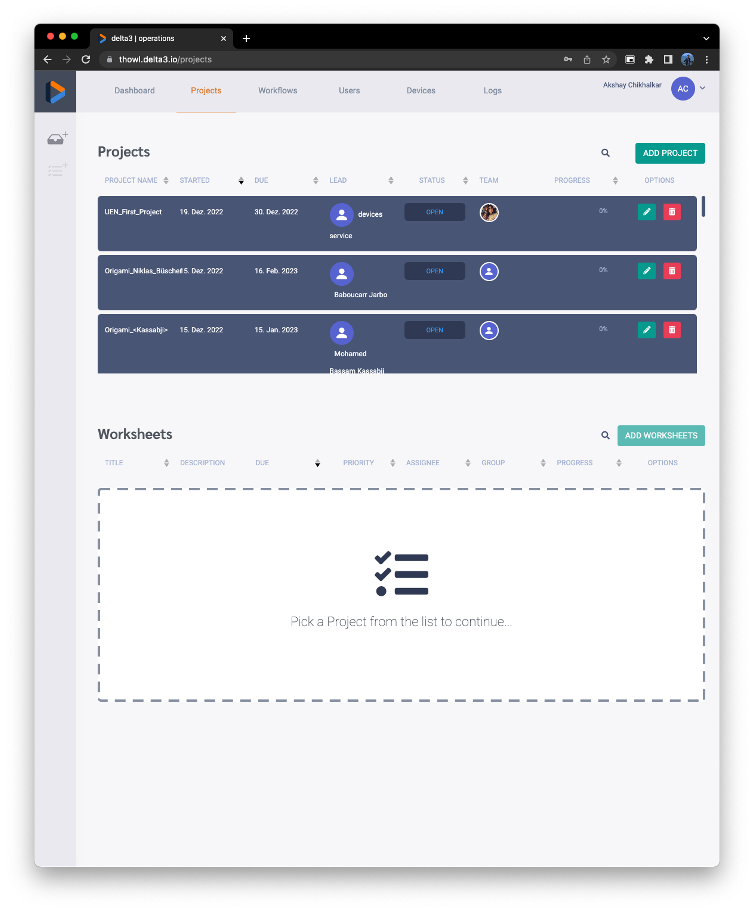
\includegraphics[width=100mm,scale=1]{./images/Operation_Problem_1.png}}
        \caption{Operation Problem 1}
        \label{Operation Problem 1}
    \end{figure}  
    \begin{figure}[H]
        \centerline{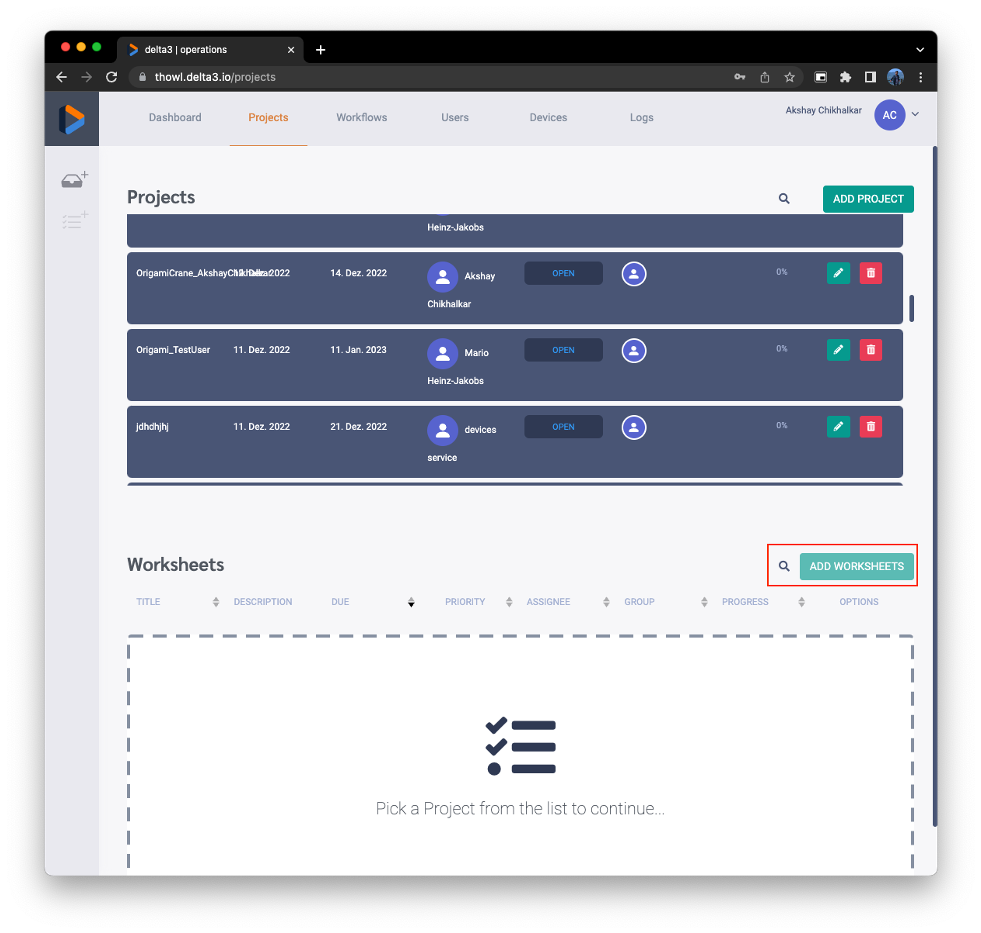
\includegraphics[width=100mm,scale=1]{./images/Operation_Problem_2.png}}
        \caption{Operation Problem 2}
        \label{Operation Problem 2}
    \end{figure}  
    \begin{figure}[H]
        \centerline{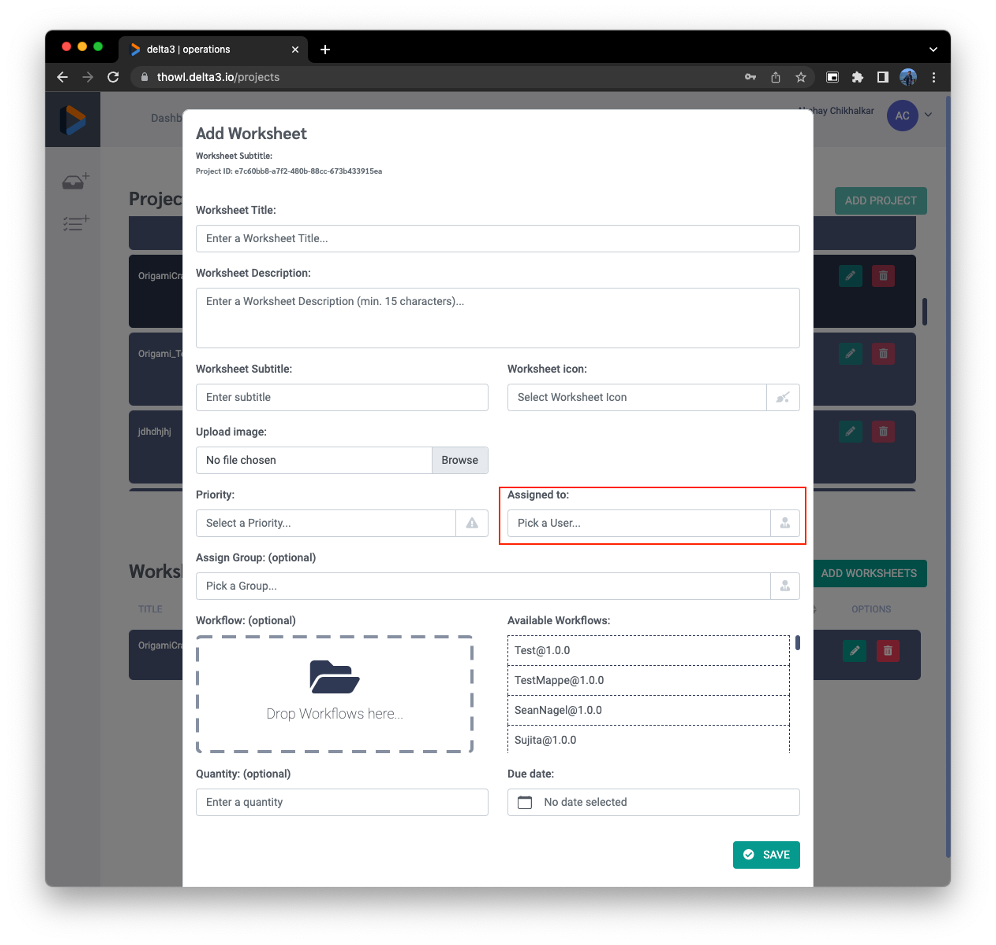
\includegraphics[width=100mm,scale=1]{./images/Operation_Problem_3.png}}
        \caption{Operation Problem 3}
        \label{Operation Problem 3}
    \end{figure}  
    \begin{figure}[H]
        \centerline{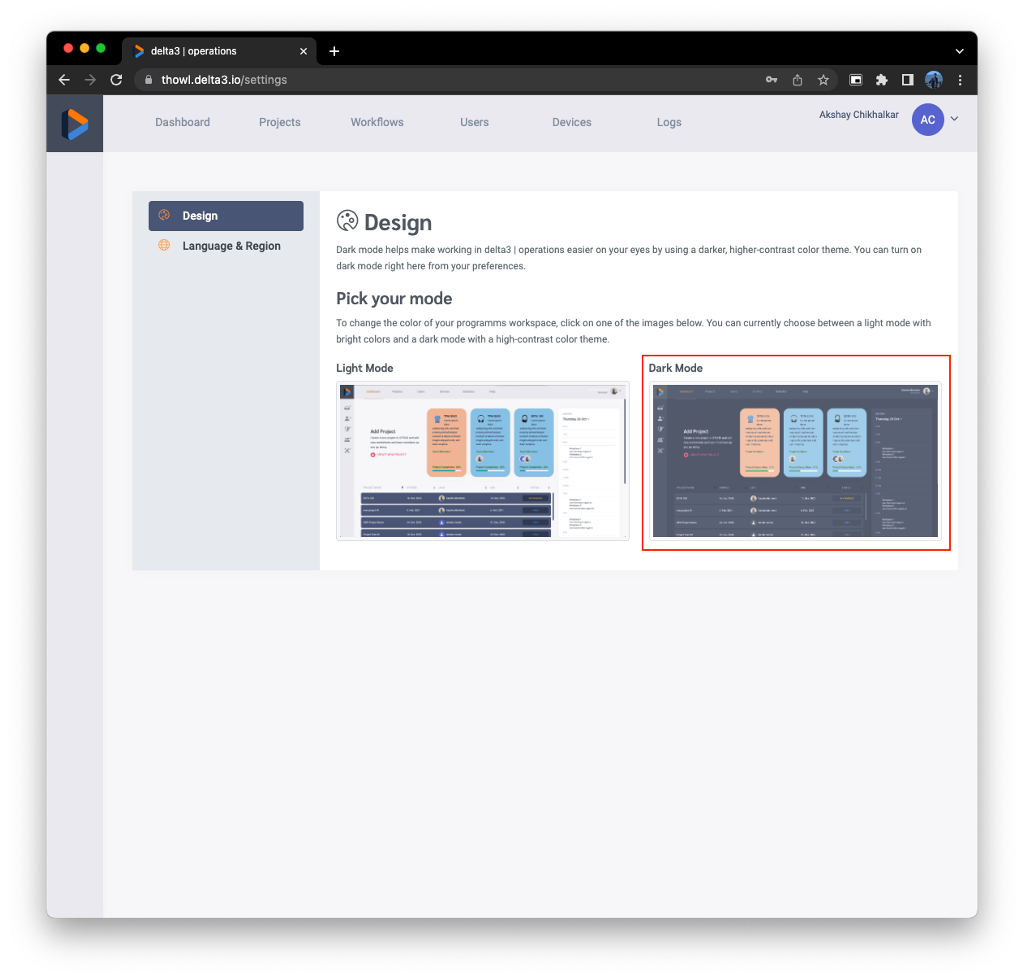
\includegraphics[width=100mm,scale=1]{./images/Operation_Problem_4.png}}
        \caption{Operation Problem 4}
        \label{Operation Problem 4}
    \end{figure}  
    \begin{figure}[H]
        \centerline{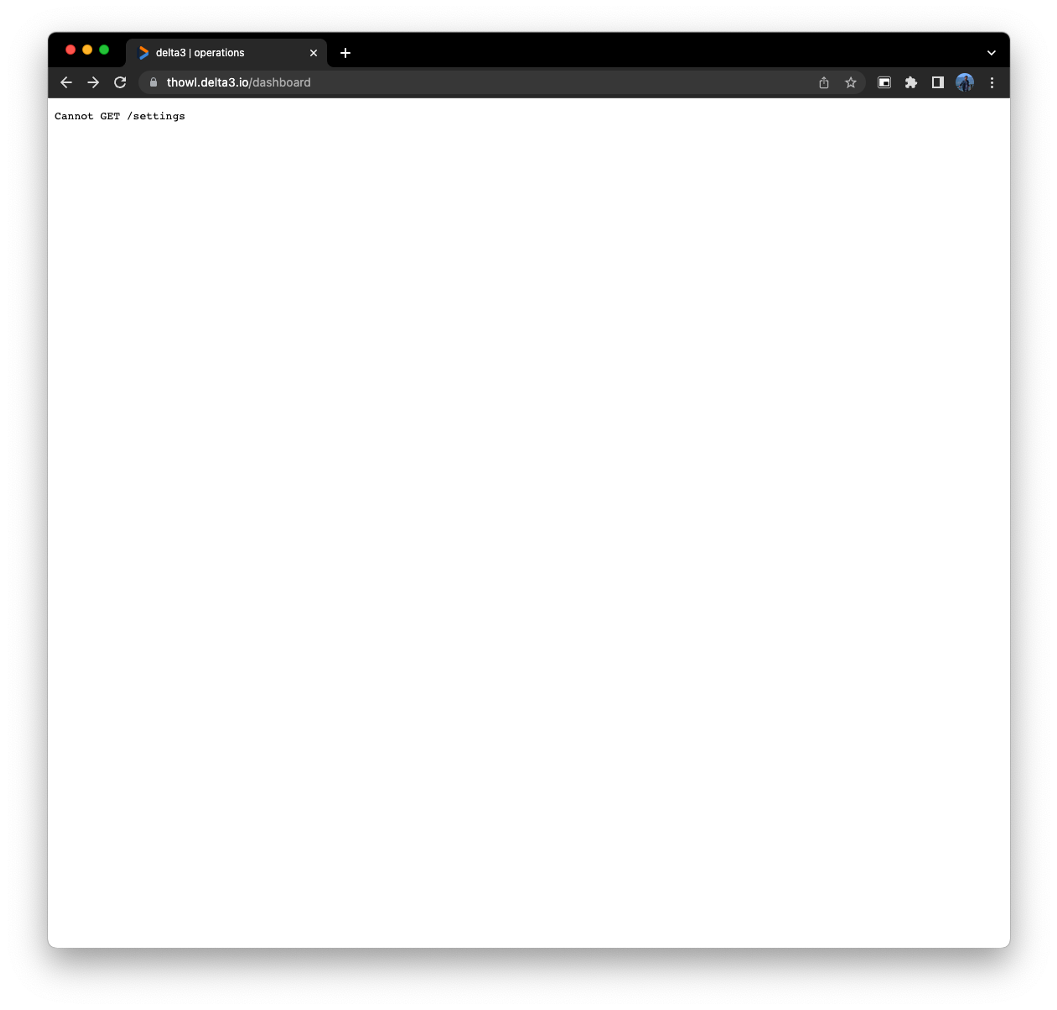
\includegraphics[width=100mm,scale=1]{./images/Operation_Problem_5.png}}
        \caption{Operation Problem 5}
        \label{Operation Problem 5}
    \end{figure}  


\newpage
\bibliographystyle{IEEEtran}
\bibliography{ref}
\end{document}